\chapter{Ecuaciones paramétricas y coordenadas polares. Las cónicas en coordenadas polares}
\chaptermark{Paramétricas y Polares}

\setlength{\parindent}{0cm}

\begin{comment}
\vspace{1cm}
\section{Uno.Uno}

\begin{tikzpicture}
	\fill [left color=red!50, right color=teal!50] (0,0) rectangle (3.5,.1);
	\fill [left color=teal!50, right color=blue!50] (3.5,0) rectangle (7.5,.1);
	\end{tikzpicture}
\vspace{0.5cm}

\vspace{1cm}
\subsection{Uno.Uno.Uno}

\begin{tikzpicture}
	\fill [left color=red!50, right color=teal!50] (0,0) rectangle (3.5,.01);
	\fill [left color=teal!50, right color=blue!50] (3.5,0) rectangle (7.5,.01);
	\end{tikzpicture}
\vspace{0.5cm}
\end{comment}


	

Podemos pensar en una curva en el plano como si se tratase de la trayectoria de una partícula cuya posición varía con el tiempo, sus coordenadas $x$ e $y$ ahora se consideran funciones de una tercera variable $t$ llamada parámetro: $\ x(t), y(t)$.

\begin{figure}[H]
	\centering
	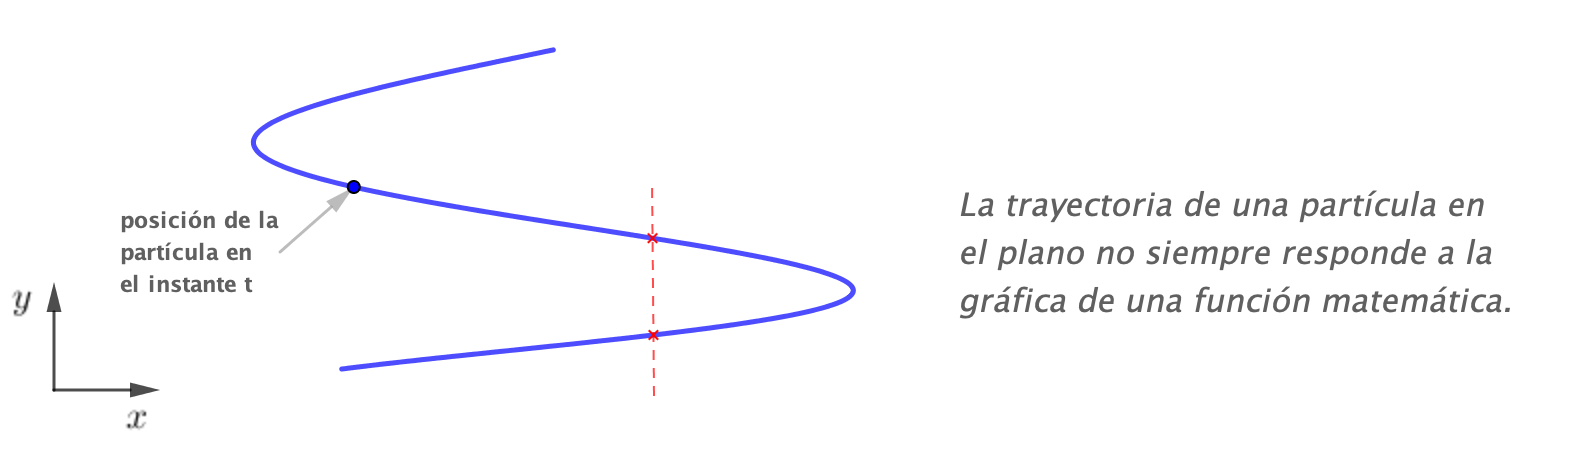
\includegraphics[width=.8\textwidth]{img-polares/polares01.png}
	\end{figure}

\vspace{-5mm}
En la figura, para una $x$ dada existe más de un valor de $y$, una recta vertical corta más de una vez a la curva por lo que no se trata de una verdadera función matemática.\footnote{Ver apartado 2.1, \textit {'Funciones reales de variable real'} del libro \textit`` {Cálculo infinitesimal \begin{scriptsize}(avanzado)\end{scriptsize} para bachillerato''}, de Ignacio Vallés Oriola, \textit{`Estrategia de la línea vertical'}. En  $\ \ $\textcolor{blau}{http://igvaori.github.io}}

Las ecuaciones paramétricas son útiles para describir curvas que no sean necesariamente funciones.

\section{Ecuaciones paramétricas}
\vspace{-5mm}

\begin{tikzpicture}
	\fill [left color=red!50, right color=teal!50] (0,0) rectangle (3.5,.1);
	\fill [left color=teal!50, right color=blue!50] (3.5,0) rectangle (7.5,.1);
	\end{tikzpicture}



\begin{cuadro-naranja}
\textbf{Curva paramétrica}: permite representar una curva en el plano mediante valores que recorren un intervalo real con una nueva variable llamada \emph{parámetro}, las coordenadas de cada punto serán funciones de este parámetro.
\vspace{-2mm}
$$C(x,y):\ \ x=x(t)\,;\ \ y=y(t)\, ; \quad \text{ con } t\in [a,b]\subset \mathbb R $$
\vspace{-2mm}
$(x(a),y(a))$ es el punto inicial de la curva, $(x(b),y(b))$ el punto final.
\vspace{2mm}
\end{cuadro-naranja}

Una misma curva admite distintas parametrizaciones.

\textsf{Cualquier función $\ y=f(x) \ $ puede parametrizarse de forma natural haciendo $\ x(t)=t\, ;\ \ y(t)=f(t) \ $ siendo el dominio del parámetro el mismo que el de la función.}

\vspace{5mm}
\begin{miejercicio}
	
Dibujar la curva $\ \ x=t^2\, ; \ \ y=t+1 \qquad -\infty<t<\infty$

\rule{300pt}{0.2pt}
	
	\begin{figure}[H]
	\centering
	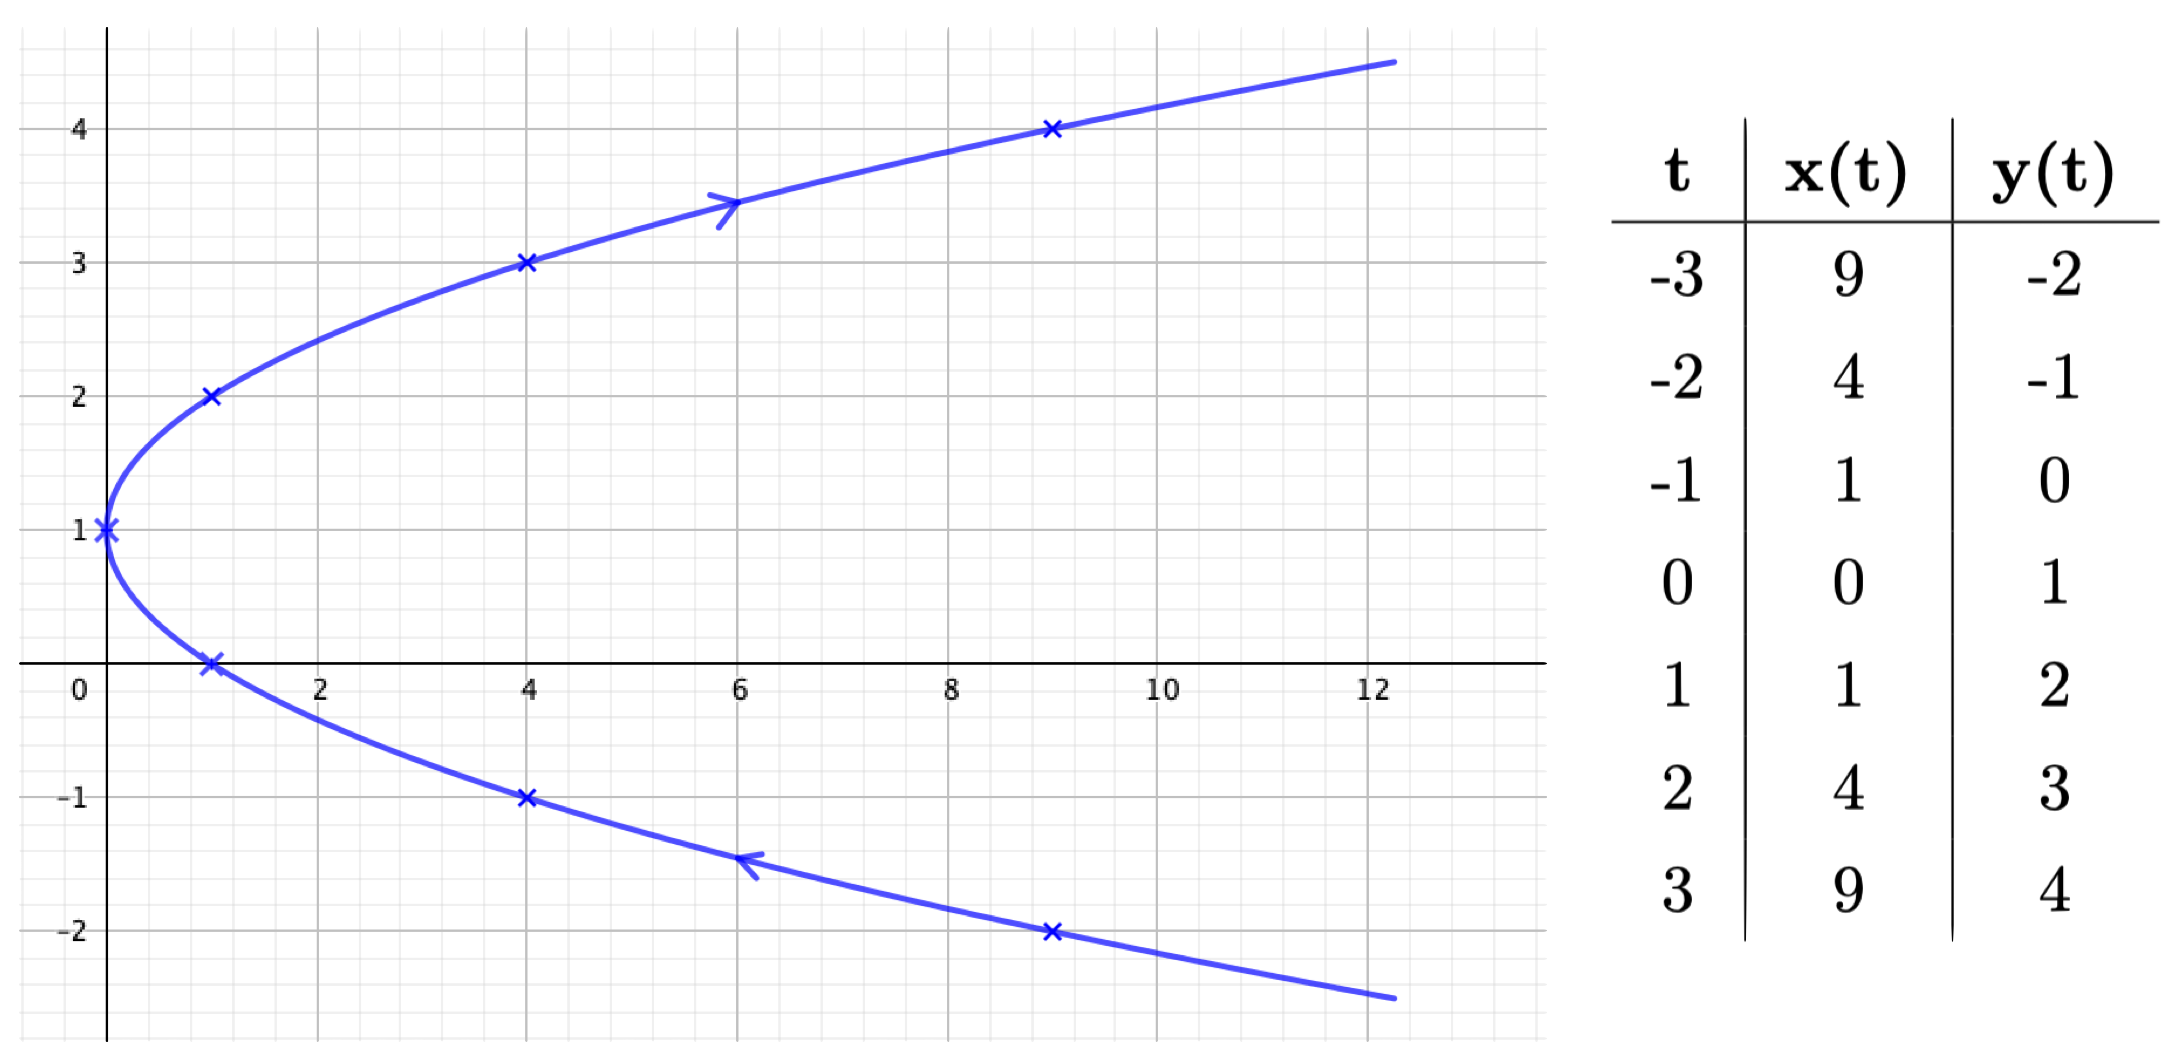
\includegraphics[width=.6\textwidth]{img-polares/polares02.png}
	\end{figure}
\end{miejercicio}

\underline{Observaciones}:
\begin{itemize}
\item Al ser el intervalo del parámetro no acotado, la curva no tiene ni punto inicial ni final. 
\item Los intervalos de tiempo de la tabla son iguales pero los puntos sobre el arco de la curva no están igualmente espaciados. \hspace{3mm} \emph{Interpretación}: La partícula reduce su velocidad a medida que se acerca al eje $y$ por la rama inferior de la curva y, una vez llegado a él en el punto (0,1), se aleja	 aumentando la velocidad por la rama superior (orientación de la curva).
\item Si eliminamos el parámetro $t$ de la ecuación de la curva (\emph{esto no siempre puede hacerse}) obtenemos la ecuación rectangular o cartesiana de la misma: 
$\ \ y=t+1 \to t=y-1 \quad\Rightarrow \quad x=(y-1)^2 \, , \ $ que es la ecuación de una parábola horizontal con vértice en $(0,1)$.

\item \emph{Compruébese} que la parametrización $\ x=m^2-2m+1\, ; \ \ y=m\ \quad -\infty<m<\infty\ $ conduce a la misma curva.
\end{itemize}



\vspace{5mm}


\begin{miejercicio}

Dibujar la curva $\ \ C(x,y):\quad x=3\cos t\, ; \ \ y=3\sin t \qquad 0\le t\le 2\pi$	

\rule{300pt}{0.2pt}

\begin{figure}[H]
	\centering
	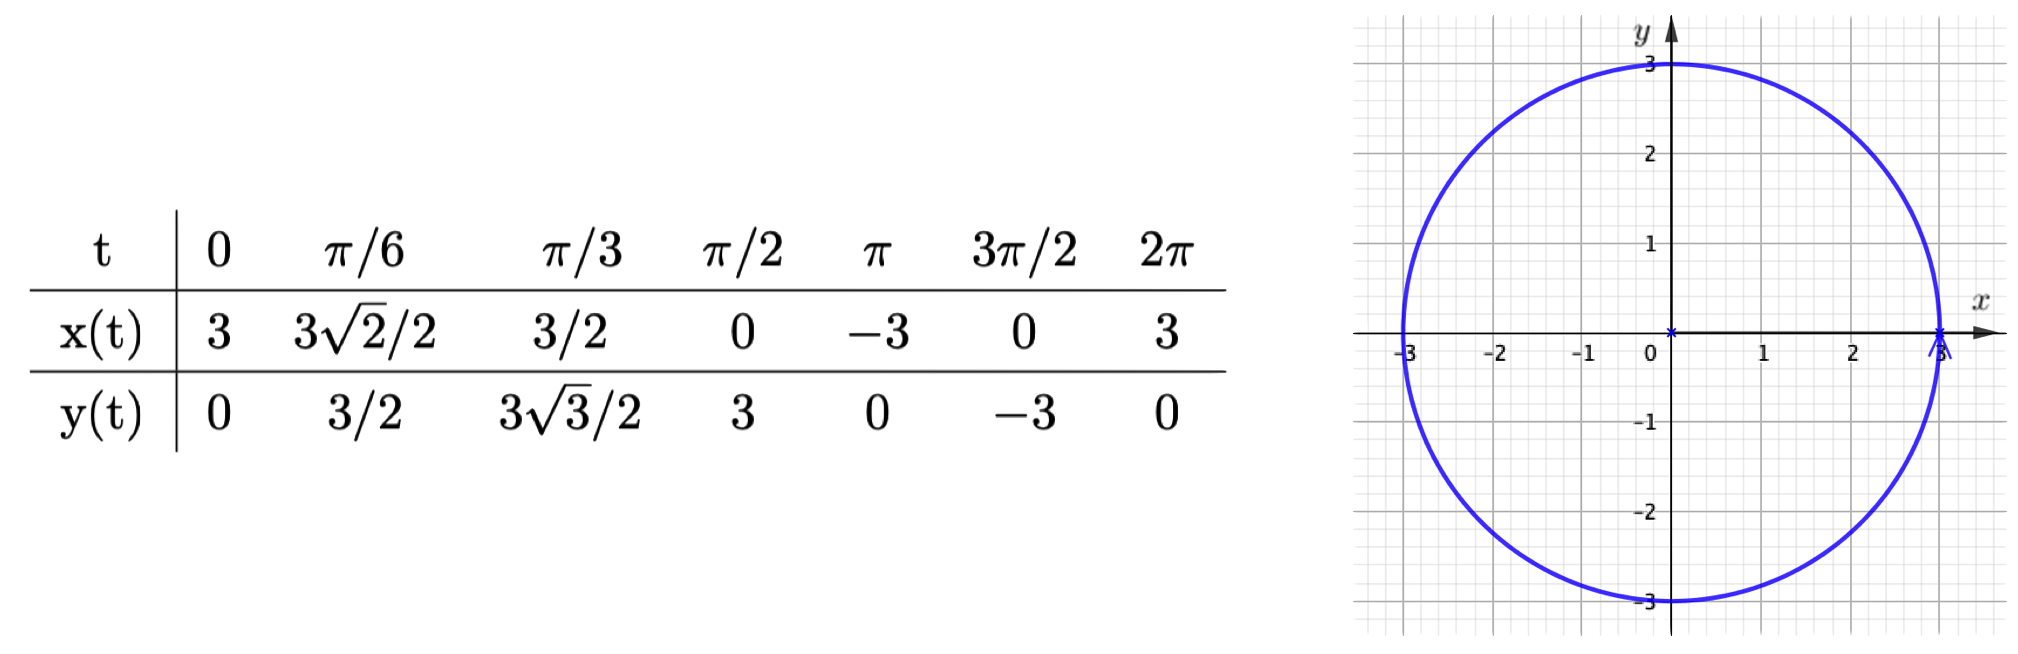
\includegraphics[width=.7\textwidth]{img-polares/polares03.png}
	\end{figure}
\end{miejercicio}

\underline{Observaciones}:
\begin{itemize}
\item Como $\ x^2+y^2=(3\cos t)^2+(3\sin t)^2=9(\cos^2 t+\sin^2 t)=9=3^2\, , \ $ se trata de la ecuación de una circunferencia de radio $3$  centrada en el origen de coordenadas.	
\item La curva empieza y acaba en $(0,1)$ y da una vuelta completa a la circunferencia en sentido \emph{levógiro} (contrario a las agujas del reloj).
\end{itemize}


\vspace{5mm}


\begin{miejercicio}

Dibujar la curva $\ \ C(x,y):\quad x=t+\dfrac 1 t\, ; \ \ y=t-\dfrac 1 t \qquad t>0$	

 \rule{300pt}{0.2pt}

\begin{figure}[H]
	\centering
	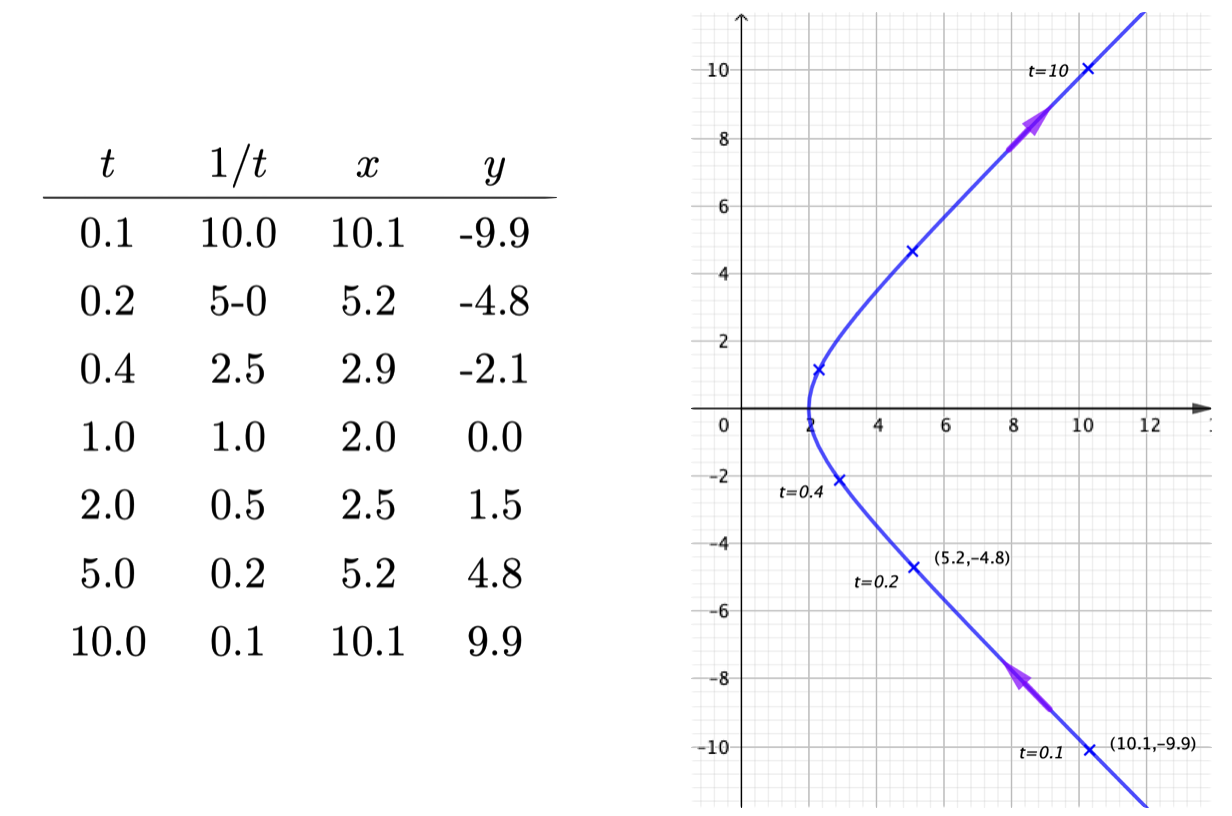
\includegraphics[width=.5\textwidth]{img-polares/polares04.png}
	\end{figure}
\end{miejercicio}

\underline{Observaciones}:
\begin{itemize}
\item Para valores pequeños de $t \ (0<t<1)$, la trayectoria está en el cuarto cuadrante y sube al primer cuadrante cuando t aumenta $(t>1)$. Al ser el dominio $]0,+\infty[$, no hay ni punto inicial ni final.
\item Eliminar el parámetro para encontrar la ecuación cartesiana de la curva es, en este caso, más difícil:

\vspace{3mm}
$\begin{cases} 
	\ x-y=\left( t+\dfrac 1 t \right) - \left( t-\dfrac 1 t \right)=\dfrac 2 t \\ 
	\  x+y=\left( t+\dfrac 1 t \right) + \left( t-\dfrac 1 t \right)=2 t 
\end{cases} \ \Rightarrow \ (x-y)(x+y)= \ \boxed{ \ \boldsymbol{x^2-y^2} \ } = \dfrac 2 t \ 2t \ \boxed { \ \boldsymbol{=4} \ }$
\vspace{3mm}

\item La hipérbola $x^2-y^2=4$ tiene en realidad otra rama, simétrica respecto del eje $y$, a la obtenida. Los puntos de nuestra curva son solo los de la hipérbola con $x=(t+1/t)>0$ al ser $t>0$, es decir, la rama derecha de la hiperbola. 
\end{itemize}

\vspace{10mm}

\begin{mipropuesto}

Dibujar la curva $\ \ C(x,y):\quad x=h+a\cos t\, ; \ \ y=k+b\sin t \qquad 0\le t\le 2\pi$	

\end{mipropuesto}


Despejando, $\quad \cos t= \dfrac{x-h}{a}\, ; \ \ \sin t= \dfrac{y-k}{b} \ \ \text { como } \ \sin^2\theta + \cos^2 \theta = 1\, , \ \forall \theta \ \therefore$

$ \dfrac{(x-h)^2}{a^2}+\dfrac{(y-k)^2}{b^2}=1 \ \ $ que es la ecuación de una elipse centrada en $(k,k)$ de semiejes $a$ y $b$.

Si $a=b=r \ \to \ $ se obtiene la ecuación de una circunferencia de radio $r$ centrada en $(h,k)$.

\begin{figure}[H]
	\centering
	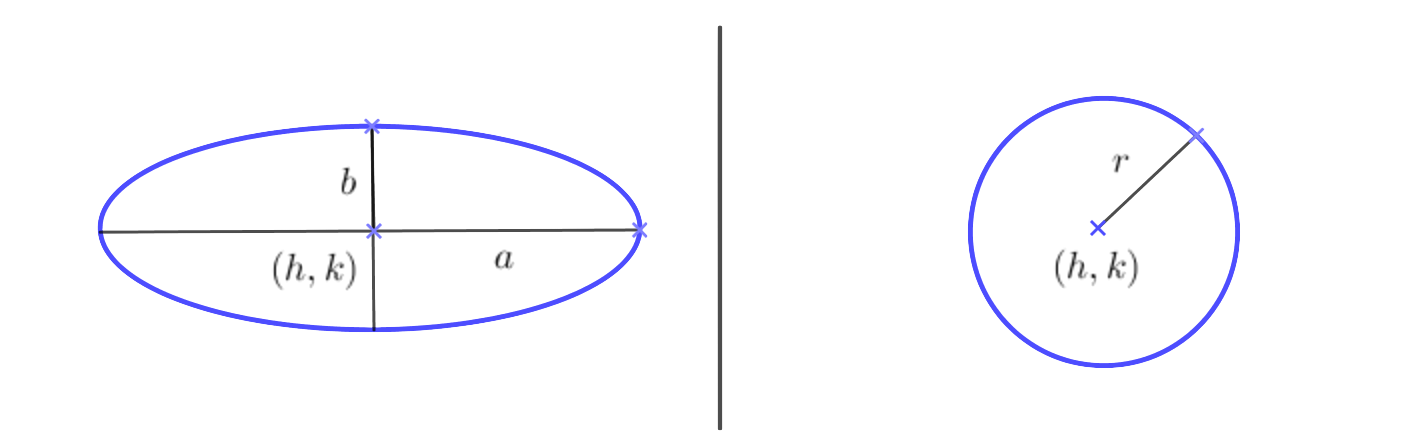
\includegraphics[width=.6\textwidth]{img-polares/polares06.png}
	\end{figure}

\begin{flushright}\textcolor{teal}{\rule{250pt}{0.2pt}}	\end{flushright}



\section{Curvas famosas \small{(en paramétricas)}}

\vspace{-5mm}

\begin{tikzpicture}
	\fill [left color=red!50, right color=teal!50] (0,0) rectangle (3.5,.1);
	\fill [left color=teal!50, right color=blue!50] (3.5,0) rectangle (7.5,.1);
	\end{tikzpicture}



\subsection{Cicloide}
\vspace{-5mm}

\begin{tikzpicture}
	\fill [left color=red!50, right color=teal!50] (0,0) rectangle (3.5,.01);
	\fill [left color=teal!50, right color=blue!50] (3.5,0) rectangle (7.5,.01);
	\end{tikzpicture}

\emph{Cicloide} es la curva que determina un punto $P$ situado sobre la superficie de un círculo de radio $r$ que gira, sin deslizamiento,  a lo largo de una recta el el plano. 

\begin{multicols}{2}
Suponemos $P$ situado sobre el origen de coordenadas cuando empieza el movimiento del círculo girando hacia la derecha. Cuando haya girado $t$ radianes, el círculo habrá recorrido sobre el eje $x$ la distancia $r\cdot t$, ya que \emph{arco=ángulo$\times$radio}	(líneas moradas en la figura).
\begin{figure}[H]
	\centering
	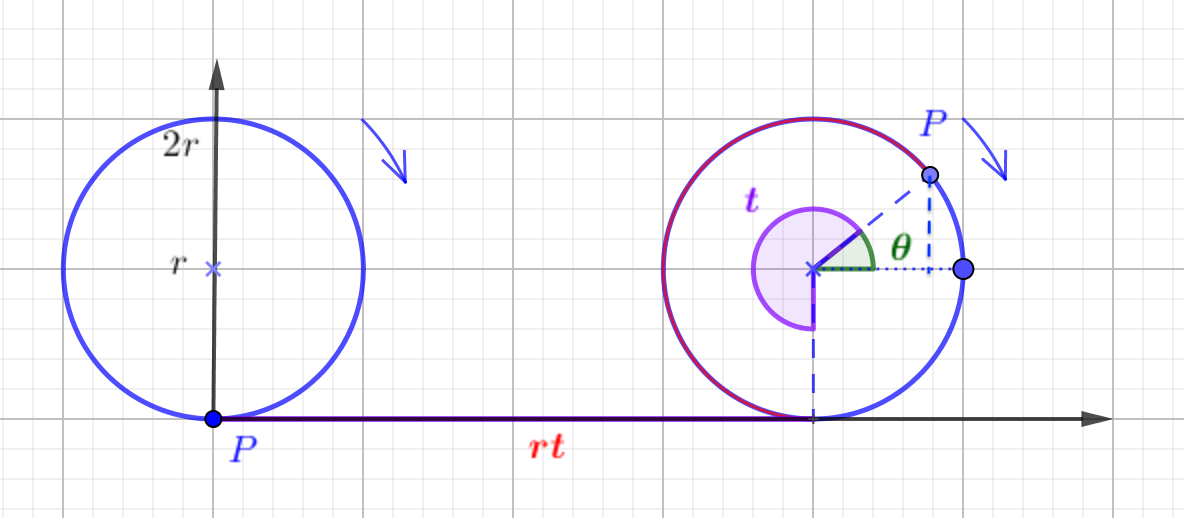
\includegraphics[width=.5\textwidth]{img-polares/polares07.png}
	\end{figure}
\end{multicols}

Las coordenadas del punto $P$ tras el giro de $rt$ radianes son:
$\quad P:\ \begin{cases} \ x=rt+r\cos \theta \\ \ y=r+r\sin \theta \end{cases}$
 
Como, de la figura $\ \ t+\theta=\dfrac{3\pi}2 \ \to \theta=\dfrac {3\pi}2-t \quad \Rightarrow \quad  \begin{cases} \ \boldsymbol{x=r(t-\sin t)} \\ \ \boldsymbol{y=r(1-\cos t)} \end{cases}$

\begin{figure}[H]
	\centering
	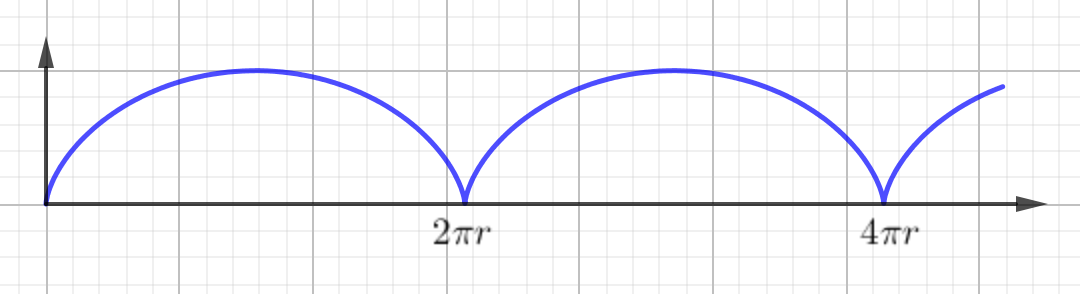
\includegraphics[width=.6\textwidth]{img-polares/polares08.png}
	\caption*{Dos primeras vueltas de la cicloide y parte de la tercera.}
	\end{figure}

\color{gris}

\vspace{5mm}
\begin{multicols}{2}
\textcolor{white}{.}\vspace{-5mm}

Si voltemos la \emph{cicloide} (cicloide invertida) se obtienen dos propiedades físicas interesantes:

\begin{figure}[H]
	\centering
	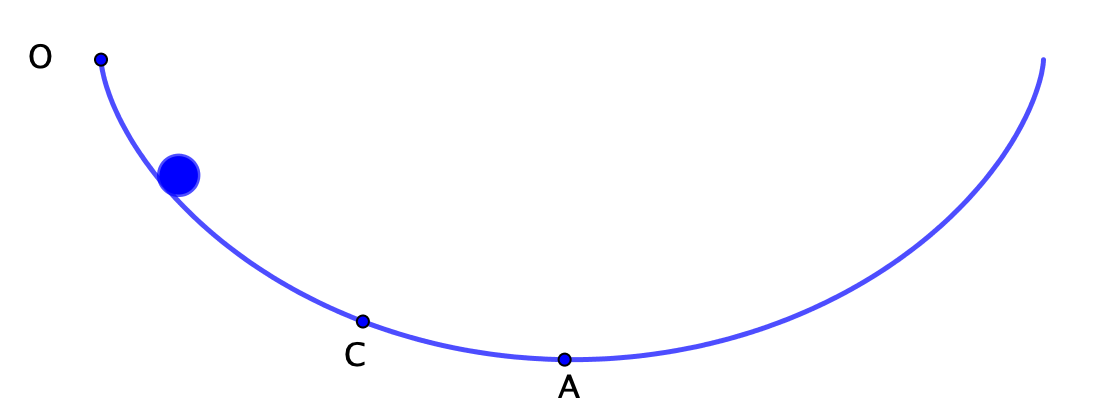
\includegraphics[width=.3\textwidth]{img-polares/polares09.png}
	\end{figure}
\end{multicols}
	
\begin{itemize}
\item De todos las curvas suaves que unen dos puntos, $O$ y $A$ a distinta altura ($A$ más bajo que $O$) la cicloide es la curva por la que una partícula sujeta solo a la fuerza de la gravedad (sin rozamiento) se deslizará en el menor tiempo posible. La \emph{cicloide} es \emph{\textbf{braquistocrona}}, curva del menor tiempo posible.
\item Aunque se suelte la partícula desde un punto intermedio del trayecto $OA$, por ejemplo desde $C$, empleará el mismo tiempo en llegar a $A$ que si la soltásemos desde $O$.	La \emph{cicloide} es \emph{\textbf{tautocrona}}, curva con el mismo tiempo, $t_{OA}=t_{CA}$ .
\end{itemize}


\begin{small}	
Un péndulo simple se define como una partícula de masa $m$ suspendida de un punto $O$ por un hilo inextensible de longitud $l$ y de masa despreciable. El periodo de un péndulo simple depende de la amplitud.

\begin{multicols}{2}
Una modificación del péndulo simple que hace que su periodo sea independiente de la amplitud consiste en hacer oscilar entre dos superficies en forma de cicliode; el hilo deja tener la forma de segmento de recta para adaptarse, en parte, a esta superficie. Es el \emph{péndulo de Huygens}, es un péndulo \textbf{\emph{isocrono}} (que se produce o se hace con un ritmo constante, con intervalos o períodos de igual duración).

\begin{figure}[H]
	\centering
	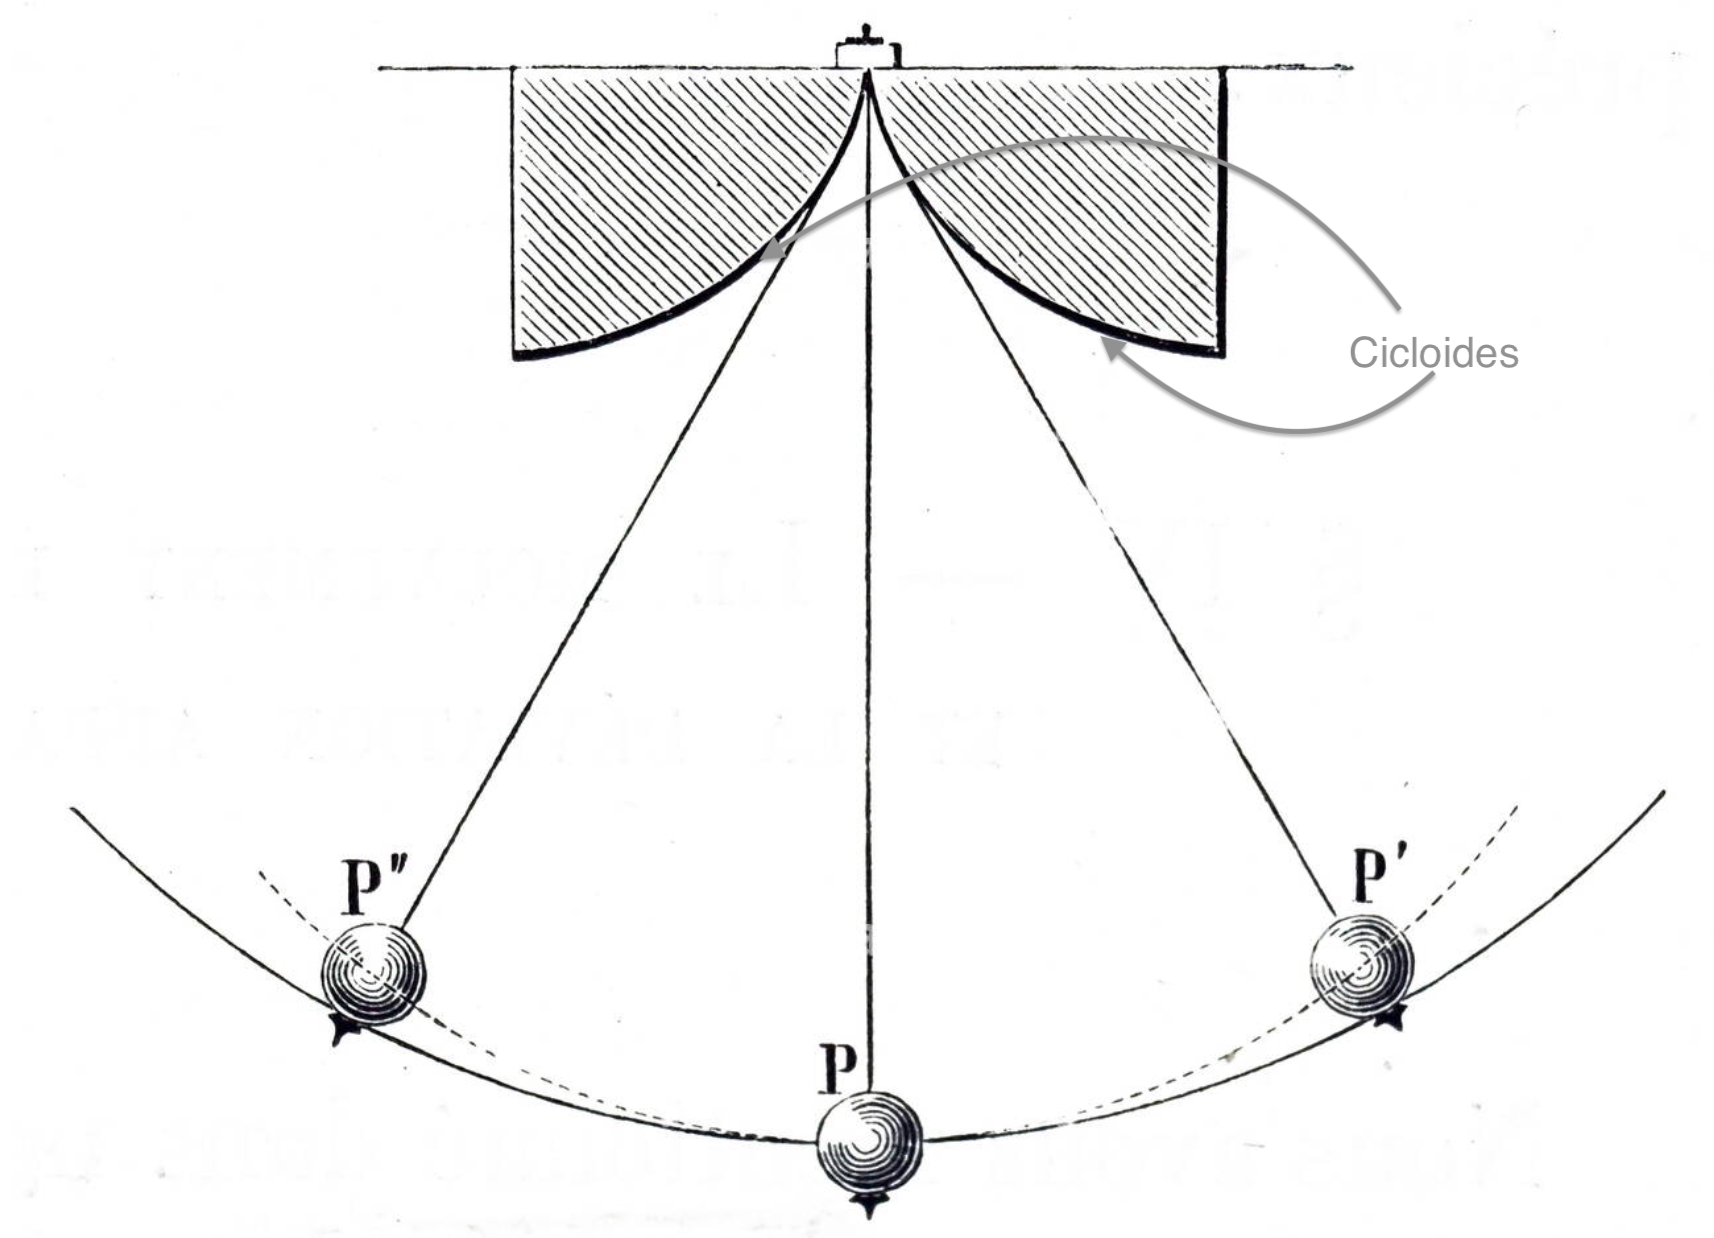
\includegraphics[width=.3\textwidth]{img-polares/polares10.png}
	\caption*{\footnotesize{Péndulo de Huygens}\normalsize{.}}
	\end{figure}
	
\end{multicols}
\end{small}

\color{black}


\subsection{Lemniscata de Bernoulli}
\vspace{-5mm}

\begin{tikzpicture}
	\fill [left color=red!50, right color=teal!50] (0,0) rectangle (3.5,.01);
	\fill [left color=teal!50, right color=blue!50] (3.5,0) rectangle (7.5,.01);
	\end{tikzpicture}


\vspace{5mm}

\normalsize{La} \emph{lemniscata} fue descrita por primera vez en 1694 por Jakob Bernoulli como la modificación de una elipse. 
\begin{multicols}{2}

Una  \emph{lemniscata} es el lugar geométrico de los puntos tales que el
producto de estas distancias a dos puntos fijos llamados  \emph{focos} es
constante. 

Bernoulli la llamó  \emph{lemniscus}, que en latín significa ``cinta colgante''. Su figura es el símbolo usado en matemáticas para representar el infinito $(\infty)$.

	\begin{figure}[H]
	\centering
	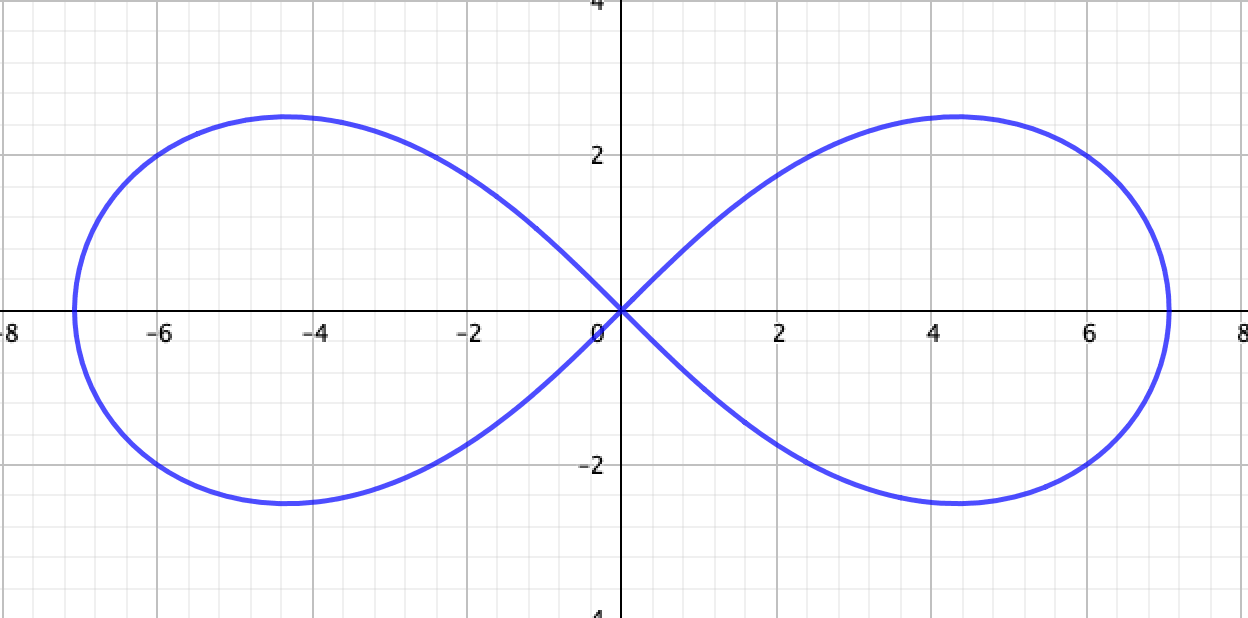
\includegraphics[width=.4\textwidth]{img-polares/polares05.png}
	\end{figure}

\end{multicols}

\subsection{Cisoide, Concoide, Nefroide, Astroide, Deltoide y Cardioide}
\vspace{-5mm}

\begin{tikzpicture}
	\fill [left color=red!50, right color=teal!50] (0,0) rectangle (3.5,.01);
	\fill [left color=teal!50, right color=blue!50] (3.5,0) rectangle (7.5,.01);
	\end{tikzpicture}

\begin{figure}[H]
	\centering
	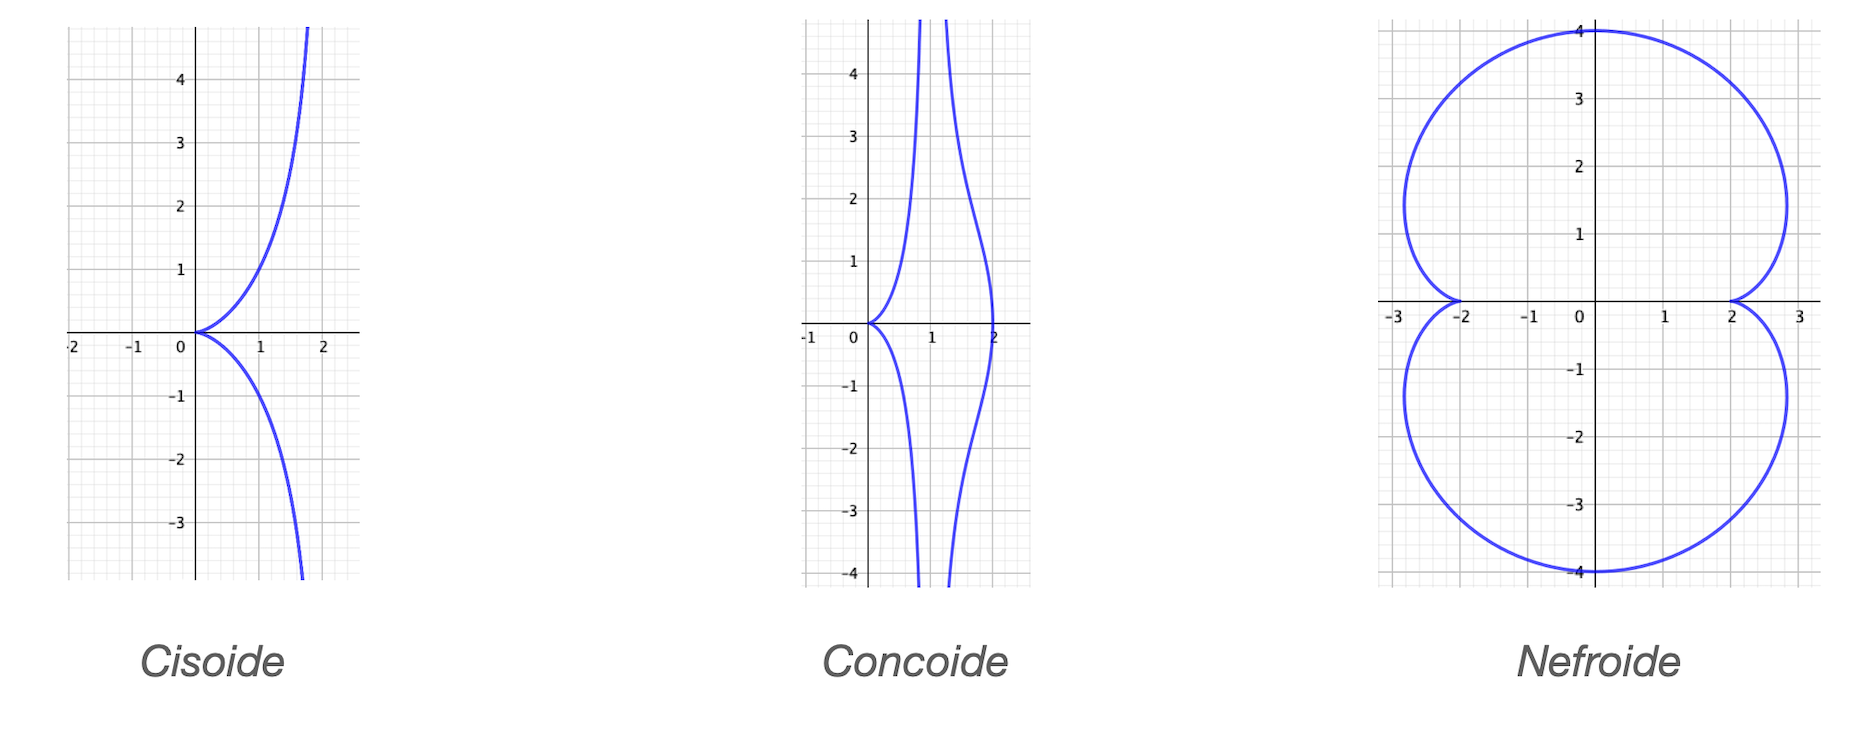
\includegraphics[width=.7\textwidth]{img-polares/polares11a.png}
	\end{figure}
\vspace{-5mm}	
\begin{figure}[H]
	\centering
	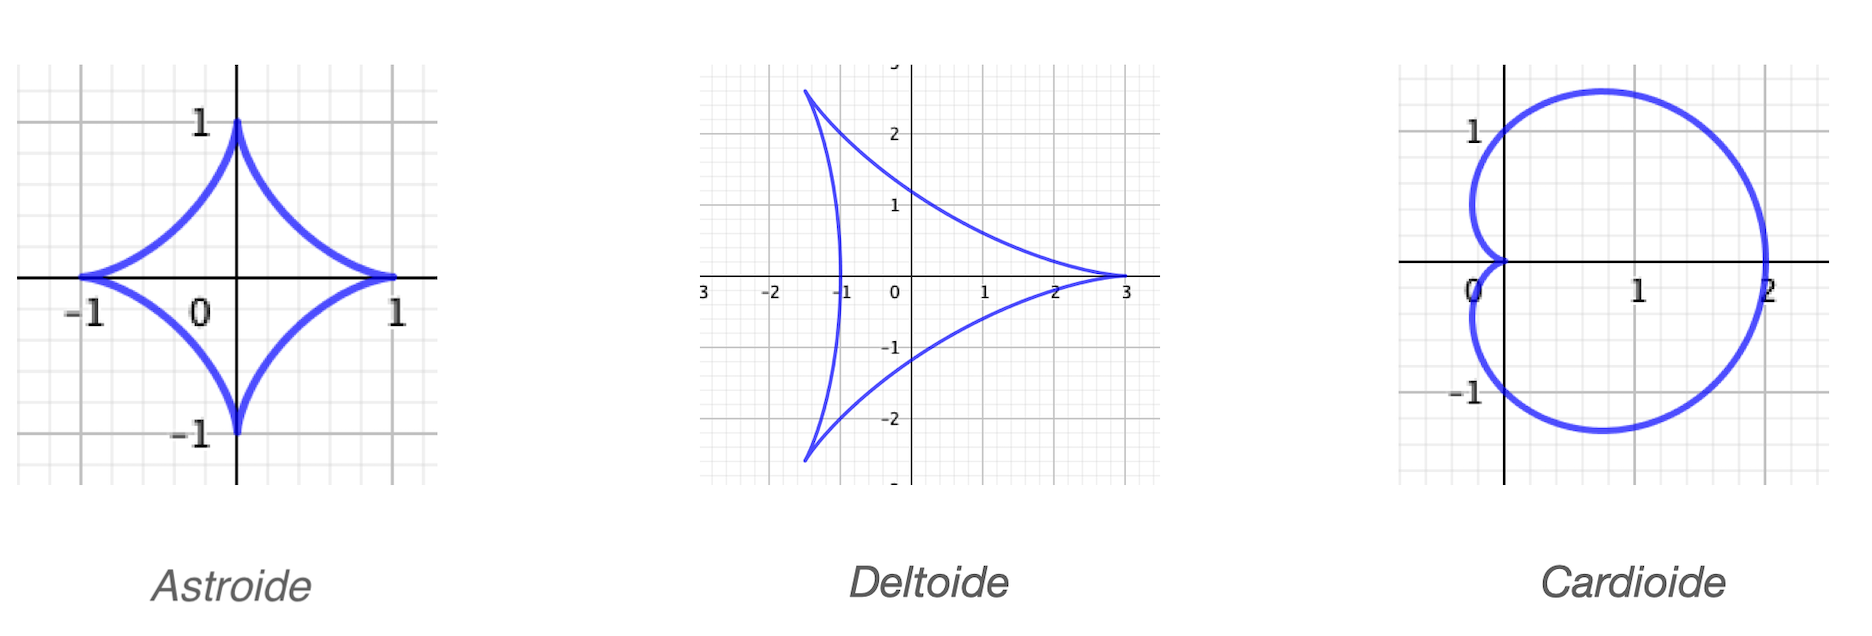
\includegraphics[width=.7\textwidth]{img-polares/polares11b.png}
	\end{figure}


\begin{table}[H]
\scriptsize
\centering
\begin{tabular}{|l|l|l|}
\hline
\multicolumn{1}{|c|}{\textbf{Cisoide}} & \multicolumn{1}{c|}{\textbf{Concoide}} & \multicolumn{1}{c|}{\textbf{Nefroide}} \\ \hline
$x=2\sin^2 t;\   y=2\sin^3 t/\cos t$ & $x=1+\cos t;\ y=\sin t + \tan t$ & $x?3\cos t-\ cos (3t);\ y=4 \sin^3 t$ \\ \hline
\multicolumn{1}{|c|}{\textbf{Astroide}} & \multicolumn{1}{c|}{\textbf{Deltoide}} & \multicolumn{1}{c|}{\textbf{Cardioide}} \\ \hline
$x=\cos^3 t;\ y=\sin^3 t$ & $x=2\cos t+\cos(2t);\ y= 2\sin t-\sin(2t)$ & $x=(\cos t+1)\cos t;\ y=(\cos t+1)\sin t$ \\ \hline
\end{tabular}
\end{table}

%\vspace{5mm} 
Otras curvas en paramétricas, dibujadas con el applet de geogebra \emph{'parametricas.ggb'} que se adjunta con estos apuntes.


\begin{figure}[H]
	\centering
	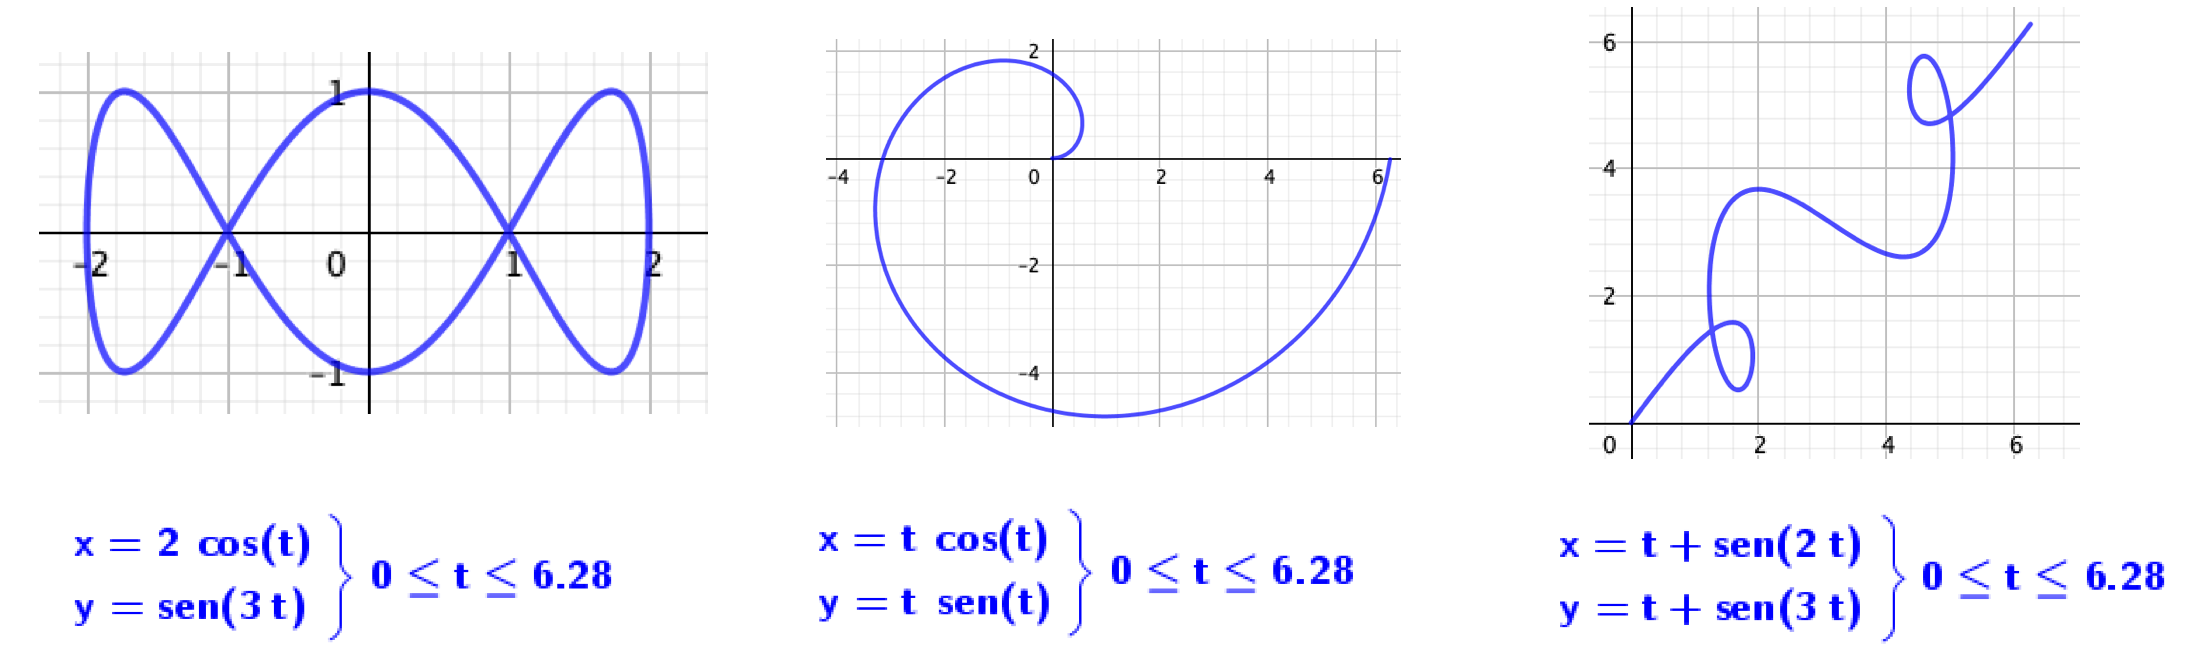
\includegraphics[width=.8\textwidth]{img-polares/polares12.png}
	\end{figure}
	
	\begin{figure}[H]
	\centering
	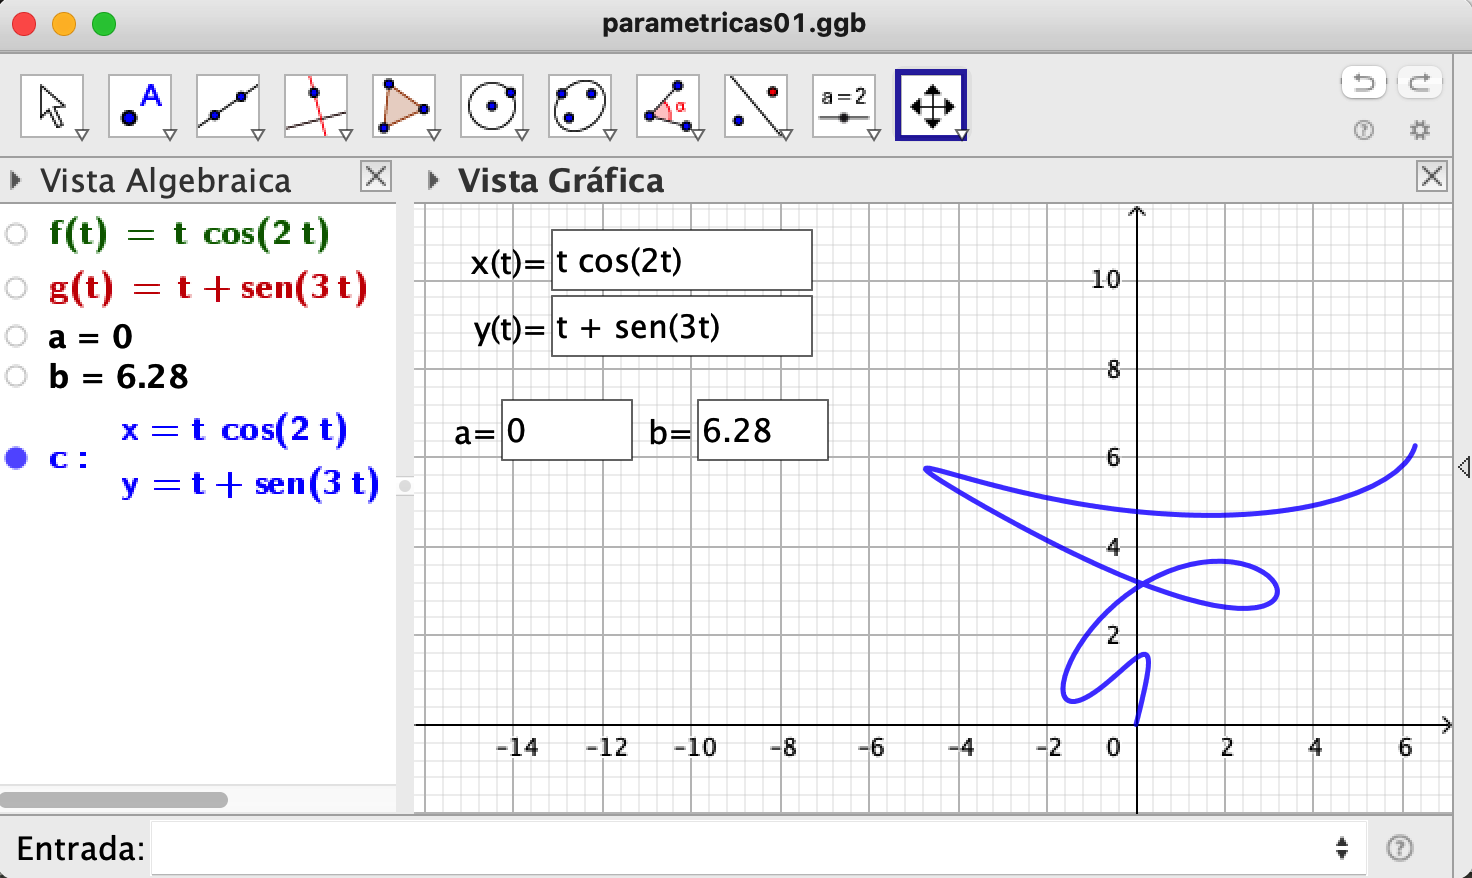
\includegraphics[width=.75\textwidth]{img-polares/polares13.png}
	\end{figure}

\begin{mipropuesto}

Determina las ecuaciones paramétricas de una partícula que empieza su movimiento en $(a,0)$	y recorre la elipse de ecuación $x^2/a^2\, + \, y^2/b^2=1$,
a) una vez en sentido levógiro; b) dos veces en sentido dextrógiro.

%\hspace{2.5cm} \rule{300pt}{0.2pt}

\end{mipropuesto}


$ \ \ a)\quad x=a\cos t\, , \ \ y=b\sin t \quad 0\le t\le 2\pi \qquad \qquad b)\quad x=a\cos t\, , \ \ y=-b\sin t \quad 0\le t\le 4\pi$


\begin{mipropuesto} 

\begin{multicols}{2}
Obtener la parametrización del segmento de recta que une los puntos $(0,2)$ con $(4,0)$ usando como parámetro el ángulo $\theta$ de la figura adjunta.
\begin{figure}[H]
	\centering
	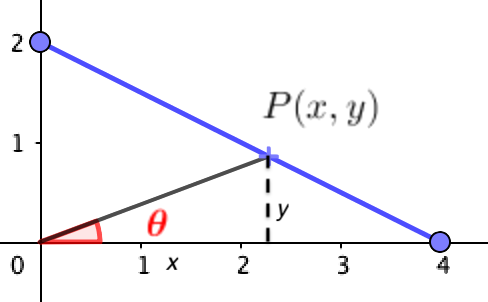
\includegraphics[width=.25\textwidth]{img-polares/polares15.png}
	\end{figure}	
\end{multicols}
\end{mipropuesto}

$\ \ \begin{cases}
\ \tan \theta =\dfrac y x \to y=x\tan \theta \\
\ r:\ \begin{cases} \ (0,2) \\ \ (4,0) \end{cases} \ y=-\dfrac 1 2 x + 2
\end{cases} \ \to \ x\tan \theta =-\dfrac 1 2 x + 2 \ \Rightarrow  \quad \begin{cases} 
 \ \boldsymbol{x=\dfrac{4}{1+2\tan \theta}}	 \\  \\ \ \boldsymbol{y=\dfrac{4\tan \theta}{1+2\tan \theta}}
 \end{cases}$


\begin{figure}[H]
	\centering
	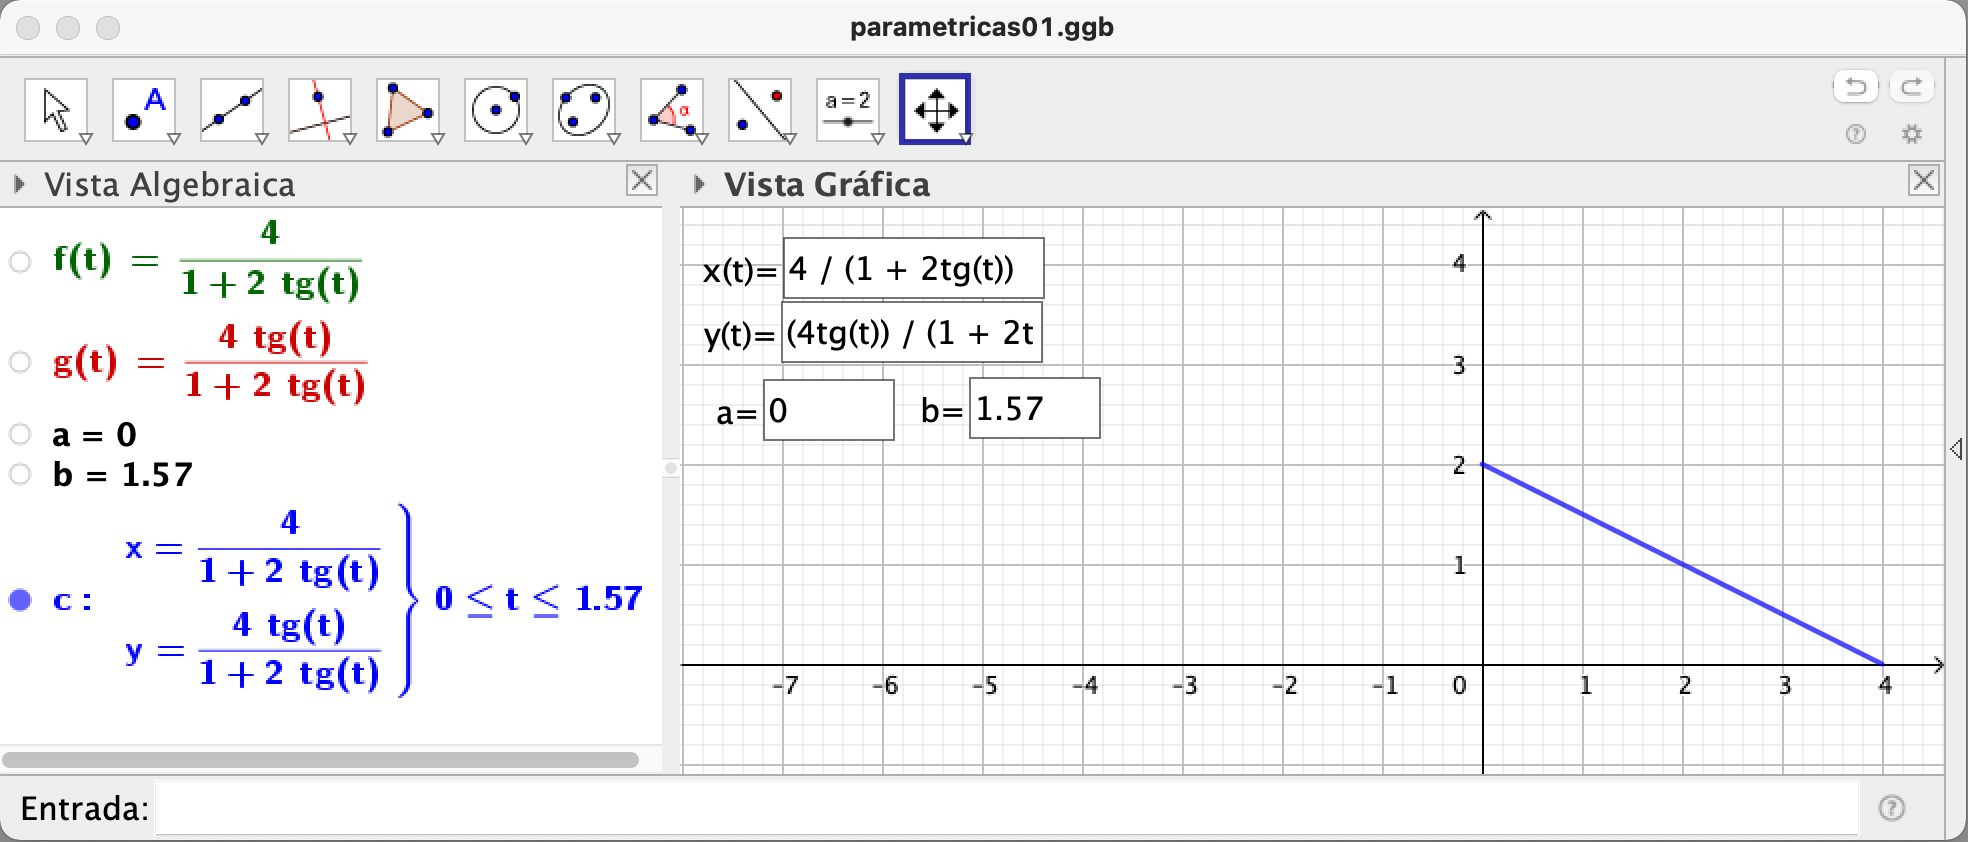
\includegraphics[width=.75\textwidth]{img-polares/polares14.png}
	\end{figure}

\vspace{-5mm}
\begin{flushright}\textcolor{teal}{\rule{250pt}{0.2pt}}	\end{flushright}\vspace{5mm}

%\vspace{5mm}
\section{Cálculo con curvas en paramétricas}

\vspace{-5mm}

\begin{tikzpicture}
	\fill [left color=red!50, right color=teal!50] (0,0) rectangle (3.5,.1);
	\fill [left color=teal!50, right color=blue!50] (3.5,0) rectangle (7.5,.1);
	\end{tikzpicture}
\vspace{0.5cm}


\large{\textbf{Recta tangente}} \normalsize{en} $(x_0,y_0):\qquad y-y_0=\eval{f'(x)}_{x_0} \cdot (x-x_0)$


En paramétricas: $\ (x(t),y(t))\ $ El punto $(x_0,y_0)$ se alcanza para algún(os) valor(es) del parámetro $t:\ \ \exists \, t_0\, / \, x(t_0)=x_0 \ \wedge \ y(t_0)=y_0$

Por otro lado, por la regla de la cadena, $\ \displaystyle \dv{y}{t}=\dv{y}{x}\dv{x}{t}$


Despejando, $ \ \ \displaystyle f'(x)=\dv{y}{x}= \dfrac{\dd y / \dd t}{\dd x / \dd t}\, , \ $ por lo que la ecuación de la recta tangente a la curva en $(x_0,t_0)$ será:

$$\subrayado{ \ \boxed{ \ \displaystyle  y-y(t_0) \ = \  \eval{\dfrac{\dd y / \dd t}{\dd x / \dd t}}_{t_0}\cdot (x-x(t_0)) \ } \ }$$


\vspace{5mm}

\begin{miejercicio}
	
Recta tangente al astroide  $\ x=\cos^3 t\, ; \ y=\sin^3 t \ $ en el punto $t=\pi/4$

\rule{300pt}{0.2pt}	

Nos piden la recta tangente a la curva cuando $\ t_0=\pi/4 \leftrightarrow x(\pi/4)=y(\pi/4)=\sqrt 2/4$ , es decir, en el punto $(\sqrt 2/4,\sqrt 2/4)$.

$ \begin{cases} 
\ x(t)=\cos^3 t \to \displaystyle \dv{x}{t}=-3\cos^2 t \sin t  
\\ \\ 
\ y(t)=\sin^3 t \to \displaystyle \dv{y}{t}=\ \ 3\sin^2 t \cos t 
\end{cases}  
\to  \ 
\displaystyle \dv{y}{x}=\dfrac{\dd y / \dd t}{\dd x / \dd t} =
\dfrac{3\sin^{\bcancel{2}} t \cancel{cos t}}{-3\\cos^{\cancel{2}} t \bcancel{\sin t}}= -\tan t$

\begin{multicols}{2}
$\quad$

Luego $\ \eval{\displaystyle \dv{y}{x}}_{t_0}= \eval{-\tan t}_{\pi/4}=-1 \ $ 

y la recta tangente buscada es:


$y-\dfrac{\sqrt{2}}{4}=-(x-\dfrac{\sqrt{2}}{4}) $

$\qquad  \qquad \to \ \ \boldsymbol{ y=-x+\dfrac{\sqrt{2}}{2} }$
\begin{figure}[H]
	\centering
	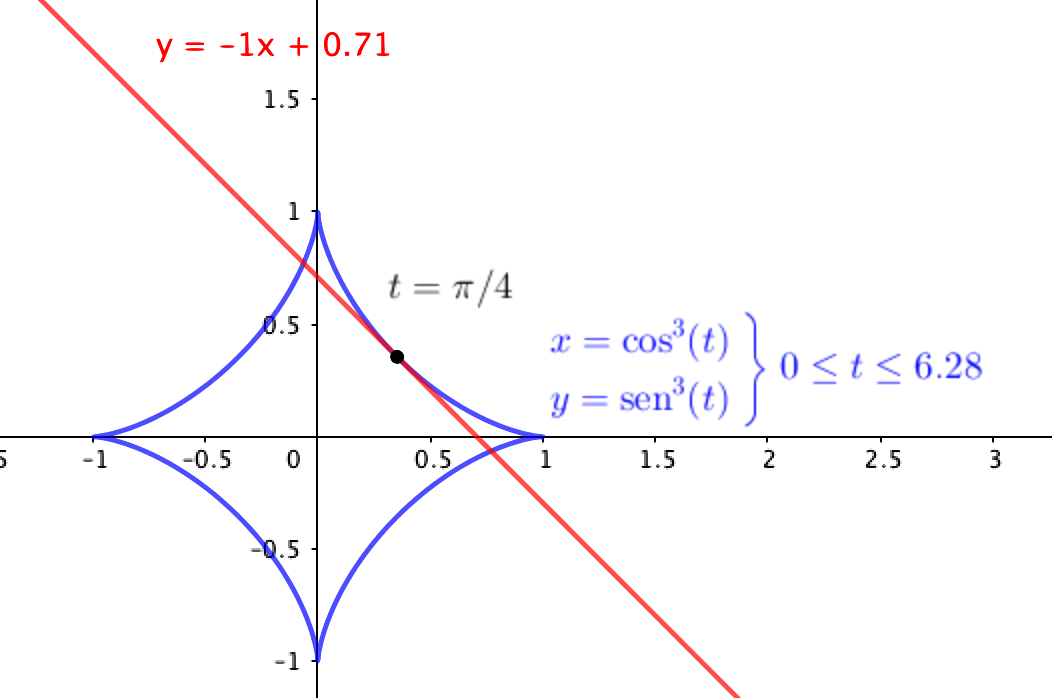
\includegraphics[width=.45\textwidth]{img-polares/polares16.png}
	\end{figure}
\end{multicols}
\vspace{1mm}
\end{miejercicio}

\vspace{5mm}


\large{\textbf{Área encerrada por una curva}}\normalsize{ $\ y=f(x)$ en} el intervalo $[a,b]$ es $\ \ A=\abs{\displaystyle \int_a^b f(x)\ \dd x}$

En paramétricas la curva es $\ (x(t),y(t))\ $ y los límites de integración serán $x=a\to t_0\,; \ x=b\to t_1$

$f(x)=y(t)\,; \quad \text{ Como } x=x(t) \ \to \ \dd x= \displaystyle \dv{x}{t} \dd t =x'(t)\dd t \ $ Así, el área será:

$$\subrayado{ \ \boxed{ \ 
\text{Área = } \abs{\displaystyle \int_{t_0}^{t_1} y(t)\, x'(t)\, \dd t} 
\ } \ }$$


\vspace{5mm}

\begin{miejercicio}

Área encerrada por el astroide $\ x=\cos^3 t\,, \ y=\sin^3 t\;\ \ t\in [0,2\pi]$

 \rule{300pt}{0.2pt}	


Por simetría, el área encerrada por el astroide es cuatro veces el área encerrada en el primer cuadrante \footnotesize{(es positiva, prescindimos del valor absoluto)}\normalsize{:}
\begin{multicols}{2}
$x=\cos^3 t \ \to \ \displaystyle \dv{x}{t}= 3\cos^2 t \sin t$

$\boldsymbol A=\displaystyle \int_0^1 y\, \dd x = 4 \int_0^{\pi/2} \sin^3 t\ 3\cos^2 t\, \sin t \ \dd t =12 \int_0^{\pi/2} \left( \dfrac{1-\cos 2t}{2} \right)^2 \left( \dfrac{1+\cos 2t}{2} \right)  \dd t = \dfrac 3 2 \int_0^{\pi/2} (1-\cos 2t -\cos^2 2t +\cos^3 2t) \dd t =$

\begin{figure}[H]
	\centering
	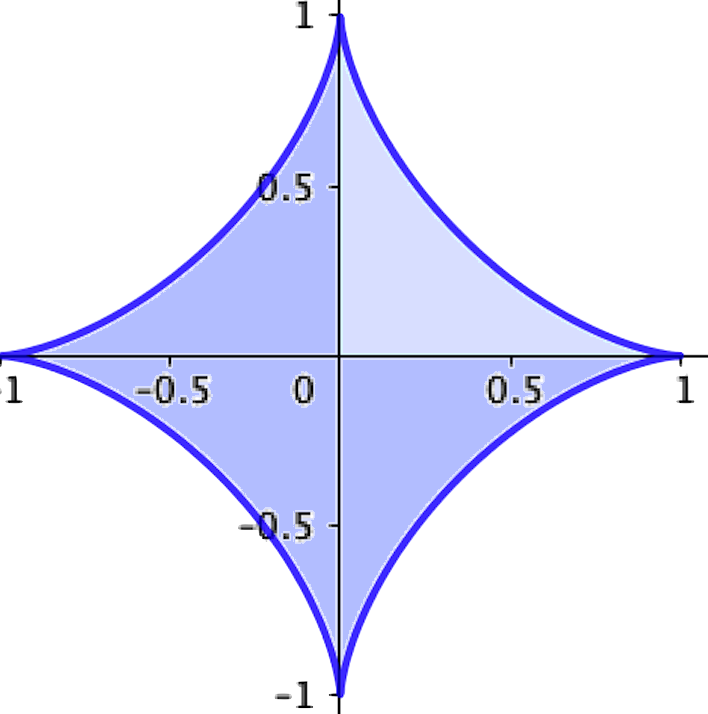
\includegraphics[width=.25\textwidth]{img-polares/polares17.png}
	\end{figure}
\end{multicols}

$\displaystyle =\dfrac 3 2 \left[
 \int_0^{\pi/2} (1-\cos 2t)\ \dd t -\dfrac 1 2 \int_0^{\pi/2} (1+\cos 2t)\ \dd t+ \int_0^{\pi/2} (1-\sin^2 t) \cos t \ \dd t \right]=$
 
 $\displaystyle =\dfrac 3 2 \left[
 \int_0^{\pi/2} (1-\cos 2t)\ \dd t -\dfrac 1 2 \int_0^{\pi/2} (1+\cos 2t)\ \dd t+ \int_0^{\pi/2} (\cos t-\sin^2 t\, \cos t ) \ \dd t \right]=$
 
 $\displaystyle =\dfrac 3 2 \left[
 \left(t-\dfrac 1 2 \sin 2t\right)- \dfrac 1 2 \left(t+\dfrac 1 2 \sin 2t\right)+ \left(\dfrac 1 2 \sin 2 t - \dfrac 1 6 \sin^3 2t\right)
  \right]_{0}^{\pi/2}= \ \boldsymbol {\dfrac {3\pi}{8}} \, \mathrm{u^2}$
\end{miejercicio}

Nota: 

Hemos usado que:  $\ \begin{cases}
 \ \sin^2 \alpha + \cos^2 \alpha &=1
 \\
 \ 	\cos^2 \alpha - \sin^2 \alpha &=\cos 2\alpha
 \end{cases} \ \ \to \ \ 
 \begin{cases}
 \ \text{sumando: } \ & \ \cos^2 \alpha = \dfrac{1+\cos 2\alpha}{2}
 \\
 \ \text{restando: } \ & \ \sin^2 \alpha = \dfrac{1-\cos 2\alpha}{2}
 \end{cases}$

\vspace{5mm}

\large{\textbf{Longitud de una arco de una curva}}\footnote{Ver apartado 8.3.3, \textit {'Cálculo de la longitud del arco de una curva'} del libro \textit`` {Cálculo infinitesimal \begin{scriptsize}(avanzado)\end{scriptsize} para bachillerato''}, de Ignacio Vallés Oriola. En  $\ \ $\textcolor{blau}{http://igvaori.github.io}}\normalsize{:}$\quad L=\displaystyle \int_a^b \sqrt{(1+f'(x))^2}\, \dd x$

En paramétricas la curva es $\ (x(t),y(t))\ $ y los límites de integración serán $x=a\to t_0\,; \ x=b\to t_1$

Como $\ x=x(t) \ \text{ e } \ y=y(t) \ \to \ \dd x=x'(t)\, \dd t \ \text{ y } \ \dd y=y'(t)\, \dd t$

$ L=\displaystyle \int_a^b \sqrt{(1+f'(x))^2}\, \dd x =
 \int_a^b \sqrt{ \left (1+ \displaystyle{\dv{y}{x}}{} \right)^2}\, \dd x =
 \int_a^b \dfrac{\sqrt{(\dd x)^2+(\dd y)^2}}{\dd x}\, \dd x= \int_a^b \sqrt{(\dd x)^2+(\dd y)^2} = \int_{t_0}^{t_1} \sqrt{x'(t)^2 \, (\dd t)^2+y'(t)^2 \, (\dd t)^2}  =  \int_{t_0}^{t_1} \sqrt{x'(t)^2+y'(t)^2} \, \dd t$


$$\subrayado{ \ \boxed{ \ \displaystyle L =  \int_{t_0}^{t_1} \sqrt{x'(t)^2+y'(t)^2} \ \dd t  = \int_{t_0}^{t_1} \sqrt{ \displaystyle \left( \dv{x}{t} \right)^2 + \left( \dv{y}{t} \right)^2  } \ \dd t \ } \ }  $$

%\vspace{5mm}

\begin{miejercicio}

Calcular la longitud del astroide: $\ x=\cos^3 t\,, \ y=\sin^3 t\;\ \ t\in [0,2\pi]$

\rule{300pt}{0.2pt}

Debido a la simetría que presenta el astroide, su longitud es 4 veces la del arco comprendido en el primer cuadrante.

$\displaystyle \left(\dv{x}{t}\right)^2=(-3\cos^2 t \sin t)^2=9\cos^4 t \sin^2 t;\qquad \left(\dv{y}{t}\right)^2=(3\sin^2 t \cos t)^2=9\sin^4 t \cos^2 t$

$\displaystyle \sqrt{\left(\dv{x}{t}\right)^2+\left(\dv{x}{t}\right)^2}=\sqrt{9\cos^2 t\sin^2 t \cancelto{1}{(\cos^2 t+\sin^2 t)}}=3|\cos t \sin t|=3\cos t\sin t \ \ (*)$

\textcolor{gris}\small{$(*):\ \ $ En el primer cuadrante, $0\leqslant t\leqslant \pi/2\, : \ \ \sin t\, \cos t\geqslant 0$}\normalsize{.}

Luego, $\ \displaystyle L=4\int_0^{\pi/2} 3 \cos t \sin t \, \dd t
=4\, \dfrac 3 2 \, \int_0^{\pi/2} \sin 2 t \, \dd t = -4\, \dfrac 3 2 \, \dfrac 1 2 \eval{\cos 2t}_0^{\pi/2}= 6\, \mathrm{u}$ 
\end{miejercicio}


\vspace{5mm}

\begin{mipropuesto}

Recta tangente a  $\ x=\sec t\, ; \ y=\tan t \ \ \ \text{ con } t\in I=]-\pi/2,\pi/2[\ $ en el punto $(\sqrt 2,1)$

\end{mipropuesto}
	
\begin{small}
$\begin{cases} \ x=sec t=\dfrac 1{\cos t}=\sqrt 2 \to \cos t =\dfrac{\sqrt 2}{2} \to \begin{cases} \ t=\pi/4 \in I \\ \ t=-\pi/4 \in I \end{cases} \\
\ y=\tan t = 1 \to \begin{cases}  t=\pi/4 \in I \\ \ t=3\pi/4 \notin I \end{cases} 
\end{cases} \hspace{-5mm} \mqty{\text{ ambas } \\ \text{ condiciones }} \to   t=\pi/4 $

Nos piden la recta tangente a la curva cuando $\ \boldsymbol{ t_0=\pi/4 \leftrightarrow (\sqrt 2,1) } $

$\begin{cases}
x(t)=\sec t=\dfrac 1{\cos t} \to \displaystyle \displaystyle \dv{x}{t}=-\dfrac 1{\cos^2 t} (-\sen t)=\dfrac{\sin t}{\cos ^2 t}
\\ \\
y(t)=\tan t \to \displaystyle \dv{y}{t}=\dfrac {1}{\cos^2 t}
\end{cases}
\displaystyle  \to  \ 
\dfrac{\dd y / \dd t}{\dd x / \dd t}=\dfrac{\dfrac {1}{\cos^2 t}}{\dfrac{\sin t}{\cos ^2 t}}=\dfrac 1{\sin t}=\displaystyle \dv{y}{x} $
\end{small}
\begin{multicols}{2}

Luego $\ \eval{\displaystyle \dv{y}{x}}_{t_0}= \eval{\dfrac{1}{\sin t}}_{\pi/4}=\dfrac{1}{\sqrt{2}/2}=\sqrt 2 \ $ 

y la recta tangente buscada es:


$y-1=\sqrt 2(x-\sqrt 2) $

$\qquad  \qquad \to \ \ \boldsymbol{ y=\sqrt{2} x-1 }$
\begin{figure}[H]
	\centering
	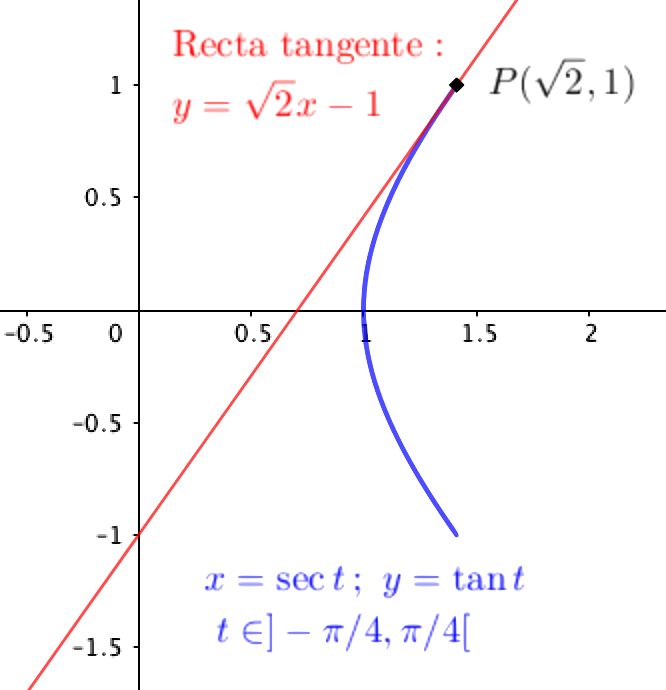
\includegraphics[width=.25\textwidth]{img-polares/polares16b.png}
	\end{figure}
\end{multicols}


\vspace{5mm}

\begin{mipropuesto}
	
 
Calcular el área bajo un arco de cicloide: $\quad x=a(t-\sin t)\, ;\ \ y=a(1-\cos t)$

\end{mipropuesto}

$A=\displaystyle \int_0^{2\pi} y\, \dd x=\int_0^{2\pi} y(t)\, \dv{x}{t}\, \dd t = \int_0^{2\pi} a(1-\cos t)\ a(1-\cos t) \ \dd t=a^2\int_0^{2\pi} (1-2\cos t+\cos^2 t)\, \dd t= a^2\int_0^{2\pi} \left(1-2\cos t+\dfrac{1+\cos 2t}{2} \right)\, \dd t= 	a^2\left[ \eval{t-2\sin t+\dfrac t 2 +\dfrac 1 4 \sin 2t }_0^{2\pi} \right.= \boldsymbol{ 3\pi \, a^2 }\ \mathrm{u}^2$
	
	\vspace{5mm}

\begin{mipropuesto}

Calcula la longitud de la curva $\ x=t^3\, ; \ \ y=3t^2/2\ $ en $\ 0\leqslant t\leqslant \sqrt 3$

\end{mipropuesto}

$L=\displaystyle \int_0^{\sqrt 3} \sqrt{(3t^2)^2+(3t)^2}\ \dd t = \int_0^{\sqrt 3} \sqrt{9t^4+9t^2}\ \dd t=\dfrac 3 2  \int_0^{\sqrt 3} 2\ t \, (t^2+1)^{1/2} \ \dd t = \dfrac 3 2 \ \eval{\dfrac{(t^2+1)^{3/2}}{3/2}}_0^{\sqrt{3}}=\eval{(t^2+1)^{3/2}}_0^{\sqrt{3}}=8-1=\ \boldsymbol 7\ \mathrm{u}$
	

\begin{flushright}\textcolor{teal}{\rule{250pt}{0.2pt}}	\end{flushright}

\section{Coordenadas polares}

\vspace{-5mm}

\begin{tikzpicture}
	\fill [left color=red!50, right color=teal!50] (0,0) rectangle (3.5,.1);
	\fill [left color=teal!50, right color=blue!50] (3.5,0) rectangle (7.5,.1);
	\end{tikzpicture}
\vspace{0.5cm}

Un \emph{Sistema de Coordenadas} en un conjunto de valores que permiten definir unívocamente la posición de cualquier punto de un espacio geométrico respecto de un punto denominado origen. 

Además del conocido \emph{Sistema de Coordenadas Cartesianas}, formado por dos ejes en el plano (tres en el espacio) mutuamente perpendiculares que se cortan en el origen y las coordenadas de un punto cualquiera vienen dadas por las proyecciones de la distancia entre el punto y el origen sobre cada uno de los ejes, también se usan los:

\begin{itemize}

\item \emph{Sistema de Coordenadas Polares} (2-dim): constituido por un eje que pasa por el origen, ahora llamado \emph{polo}. La primera coordenada es la distancia existente entre el origen y el punto, mientras que la segunda es el ángulo que forman el semieje $\mathcal {O}X+$, llamado \emph{eje polar}  y la recta que pasa por ambos puntos.



\item \emph{Coordenadas Cilíndricas} (generalización del sistema de coordenadas polares plano) y \emph{Coordenadas Esféricas}, ambos en 3-dim.
\end{itemize}


\begin{figure}[H]
	\centering
	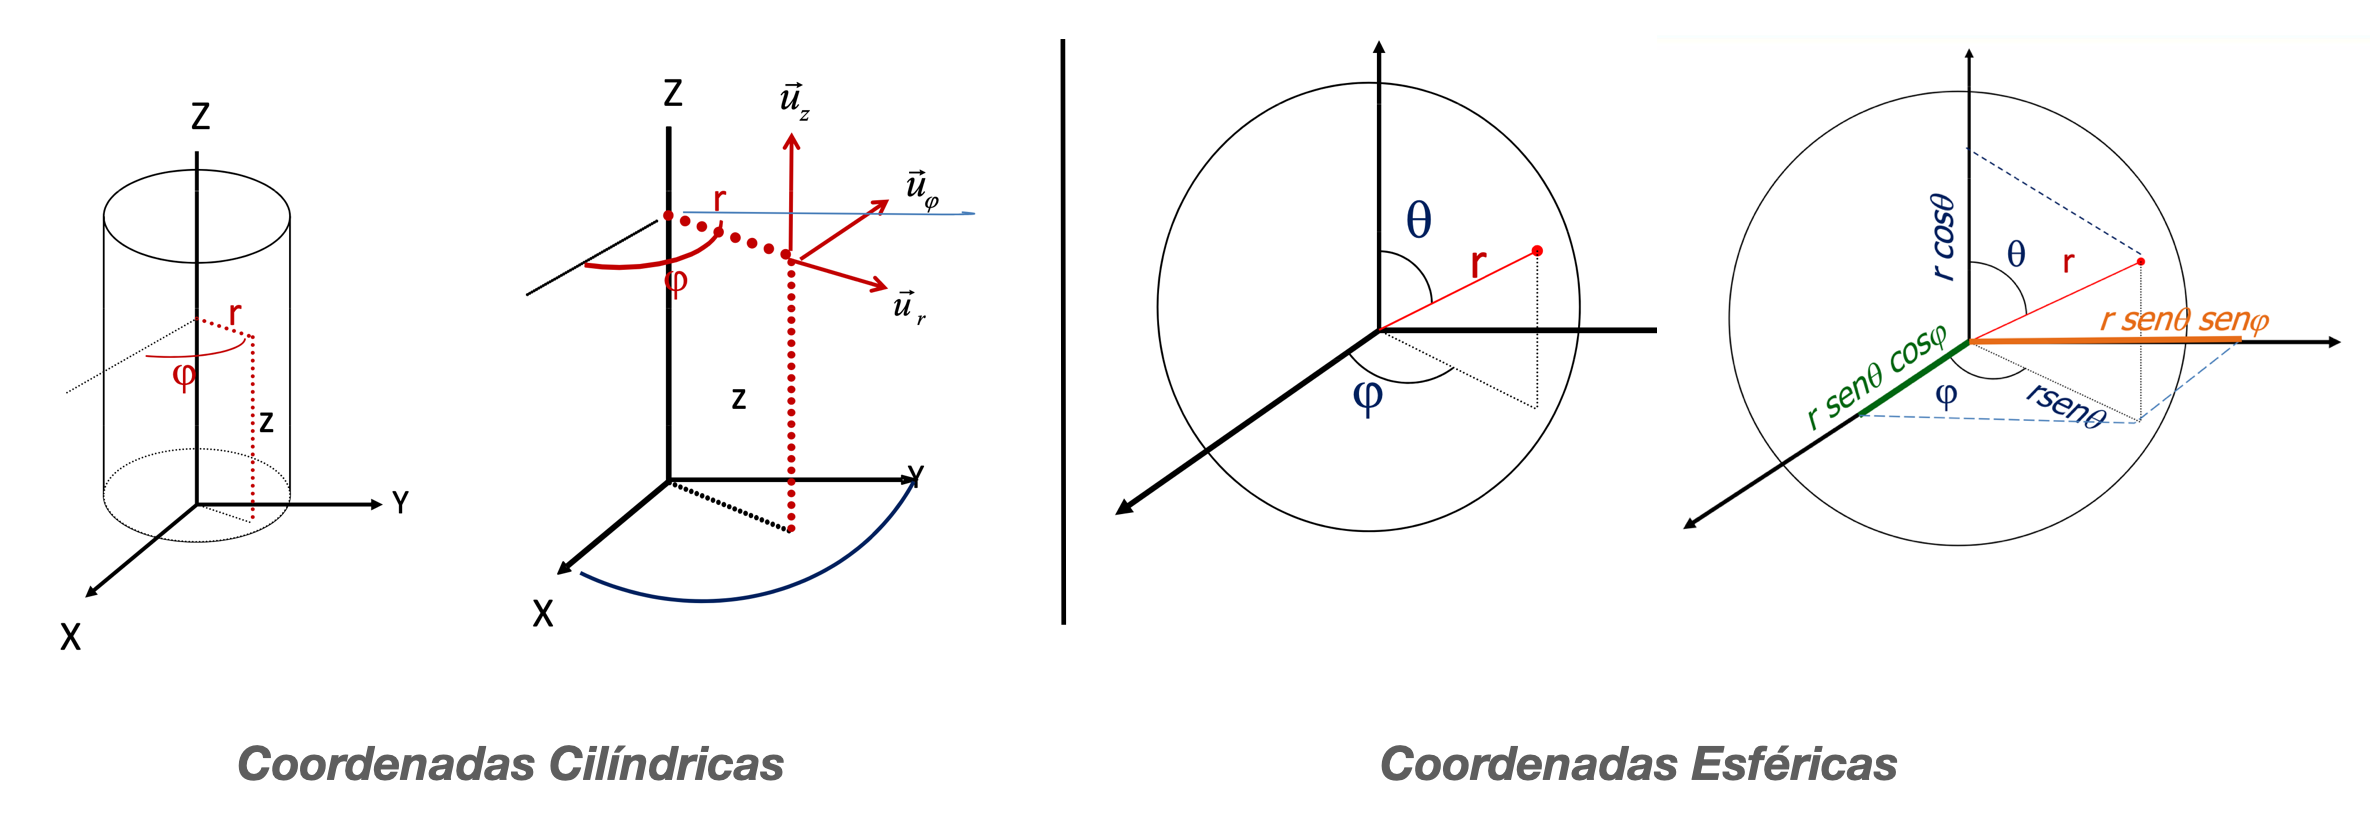
\includegraphics[width=.8\textwidth]{img-polares/polares18.png}
	\end{figure}

\textsf{Las coordenadas polares son las más adecuadas en cualquier contexto donde el fenómeno a considerar esté directamente ligado con la dirección y longitud de un punto central, como en las figuras de revolución, en los movimientos giratorios, en las observaciones estelares, etc.  Muchos sistemas físicos, tales como los relacionados con cuerpos que se mueven alrededor de un punto central que los origina, son más simples y más intuitivos de modelar usando coordenadas polares. La motivación inicial de la introducción del sistema polar fue el estudio del movimiento circular y el movimiento orbital.}

\textsf{Todos los  sistemas sometidos a una fuerza central son buenos candidatos para el uso de coordenadas polares. Algunos ejemplos son las antenas radioeléctricas o los campos gravitatorios, que obedecen a la ley de la inversa del cuadrado.}

\vspace{5mm}

\begin{figure}[H]
	\centering
	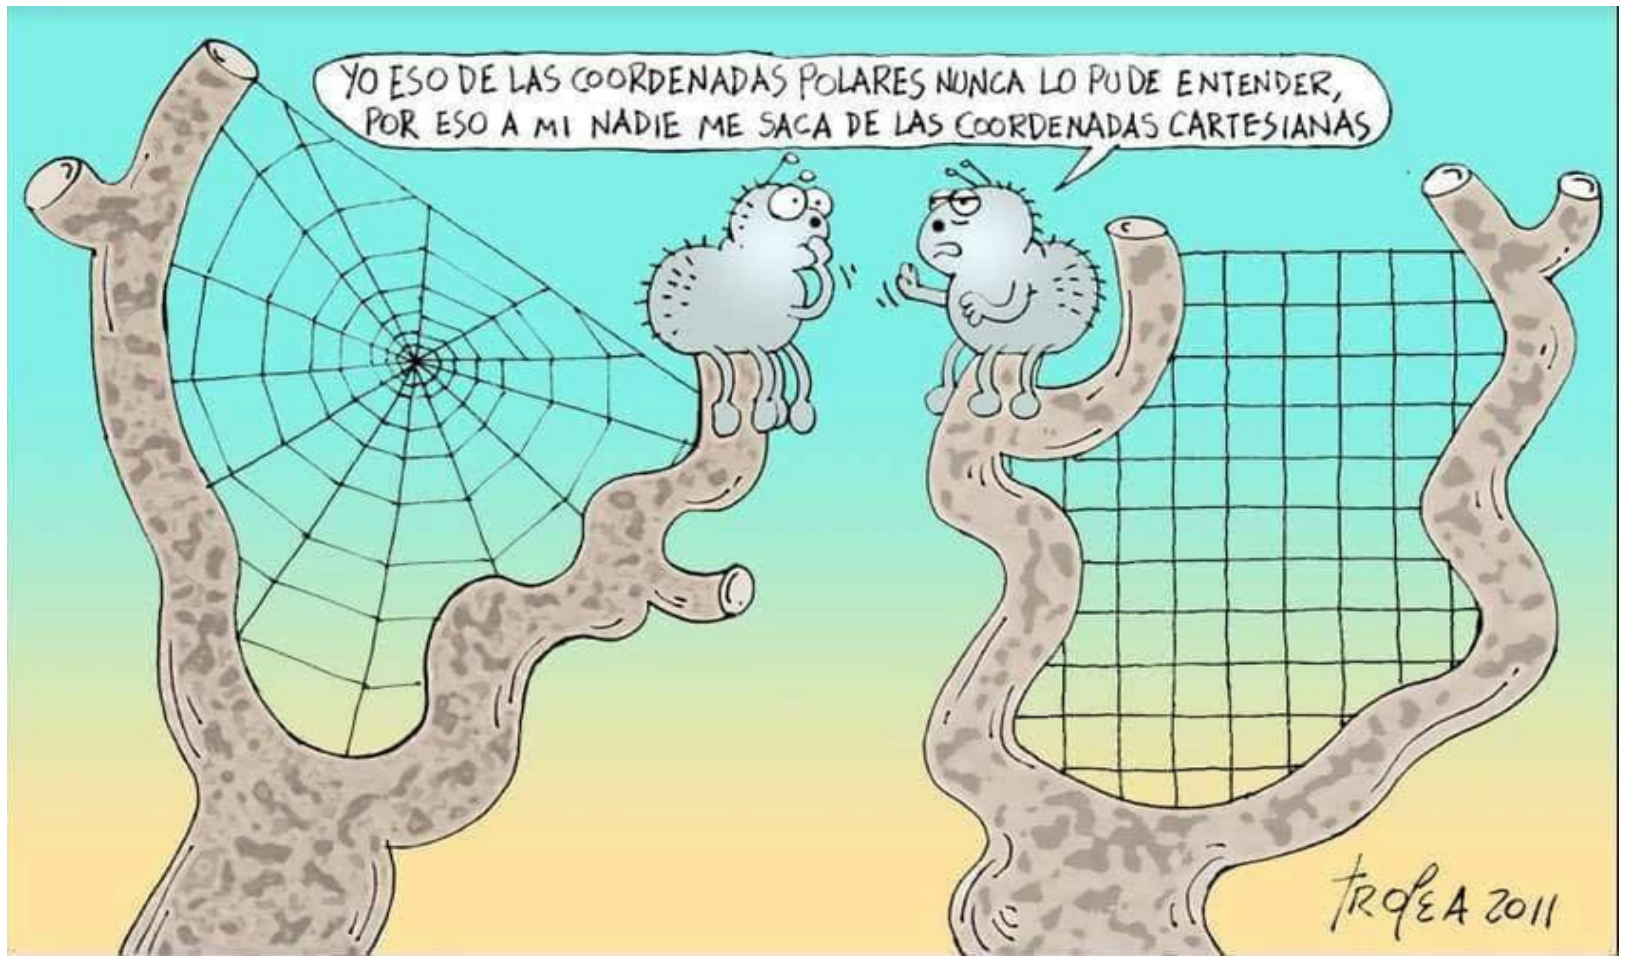
\includegraphics[width=.65\textwidth]{img-polares/polares19.png}
	\end{figure}

\vspace{5mm}

\large{\textbf{Coordenadas Polares}}\normalsize{.}

\begin{multicols}{2}
El sistema de coordenadas polares se construye dibujando una serie de circunferencias concéntricas de radio conocido a intervalos regulares, así como rayos, también a intervalos regulares, tal como se muestra abajo en la figura. Este proceso es similar al que se sigue en un sistema de coordenadas rectangulares, donde se dibujan rectas verticales y horizontales a intervalos regulares en cada caso.

\begin{figure}[H]
	\centering
	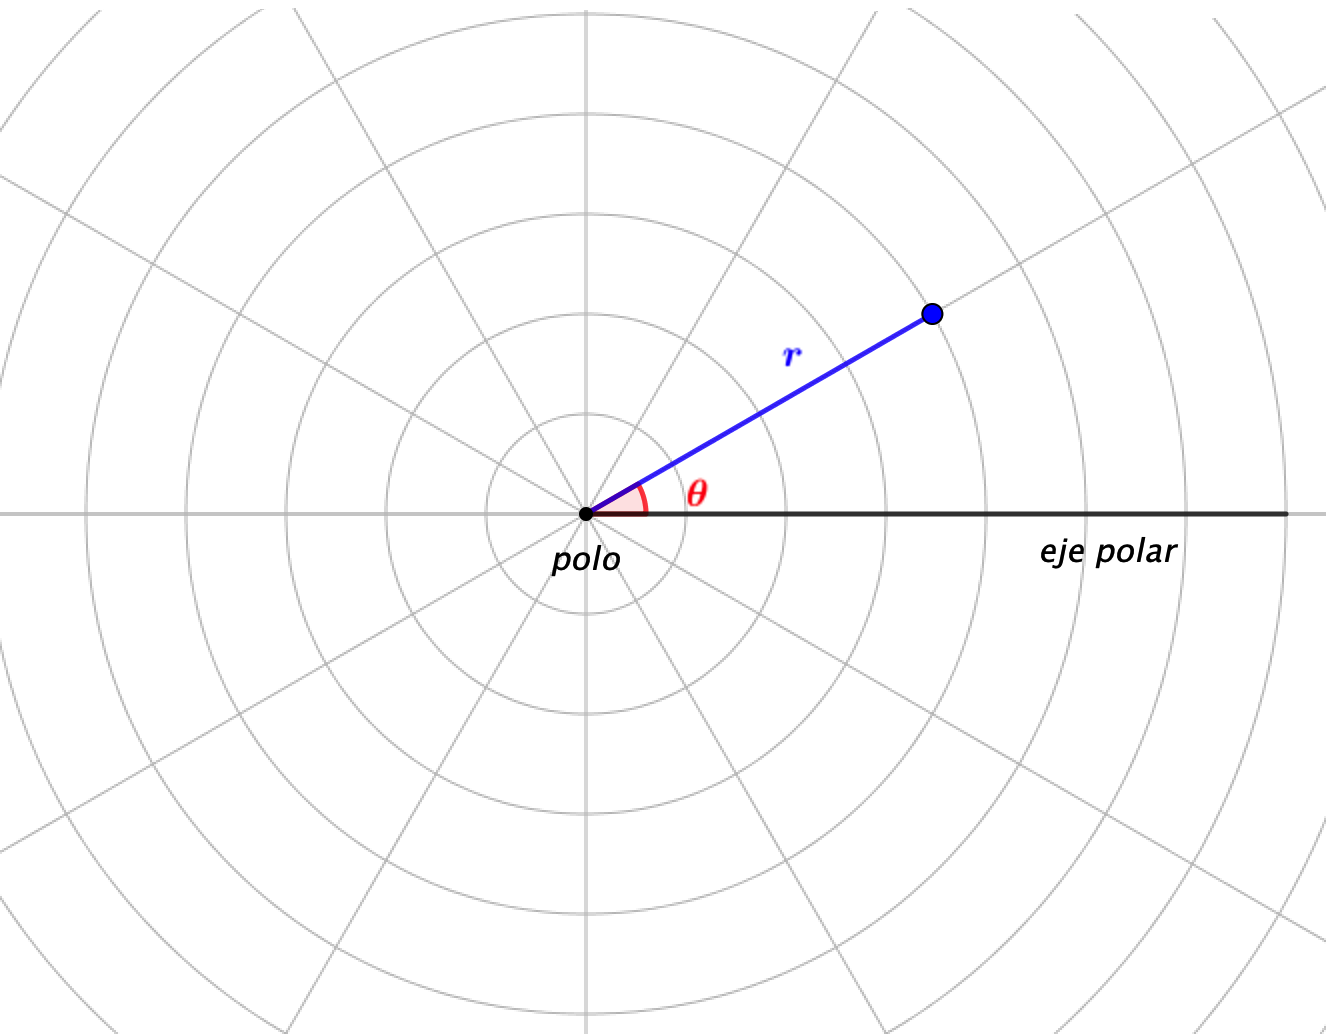
\includegraphics[width=.4\textwidth]{img-polares/polares20.png}
	\end{figure}
\end{multicols}

\vspace{5mm}

\begin{cuadro-naranja}
Un punto $P(r,\theta)$ en polares se representa por $\boldsymbol r$, la distancia de P al polo (origen) $\mathcal O$, y por $\boldsymbol \theta$, él ángulo medido desde el eje polar hasta el segmento $\overline{\mathcal {O} P}$.

\emph{Si en alguna ocasión aparece un $r<0$ se interpreta como si esta distancia estuviese medida bajo un ángulo $\theta + \pi$.}
\end{cuadro-naranja}

\begin{figure}[H]
	\centering
	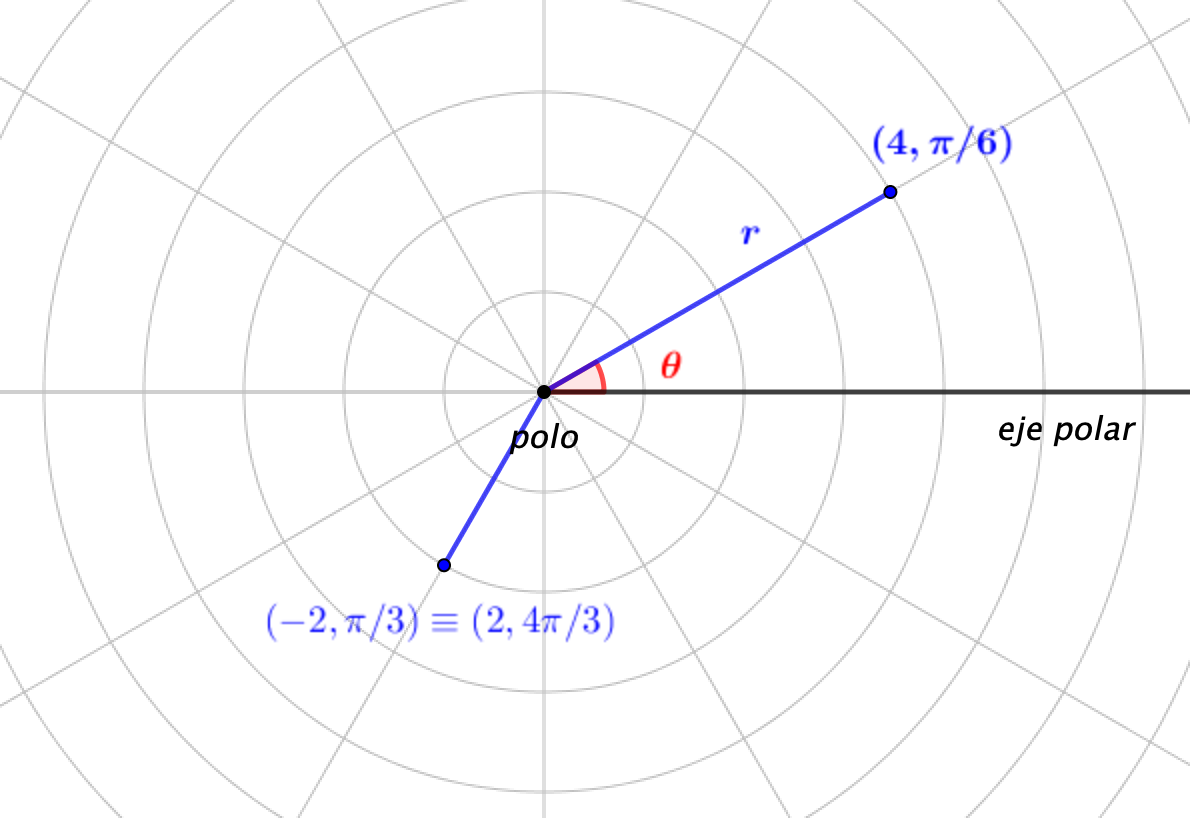
\includegraphics[width=.5\textwidth]{img-polares/polares21.png}
	\end{figure}
	
	
\begin{figure}[H]
	\centering
	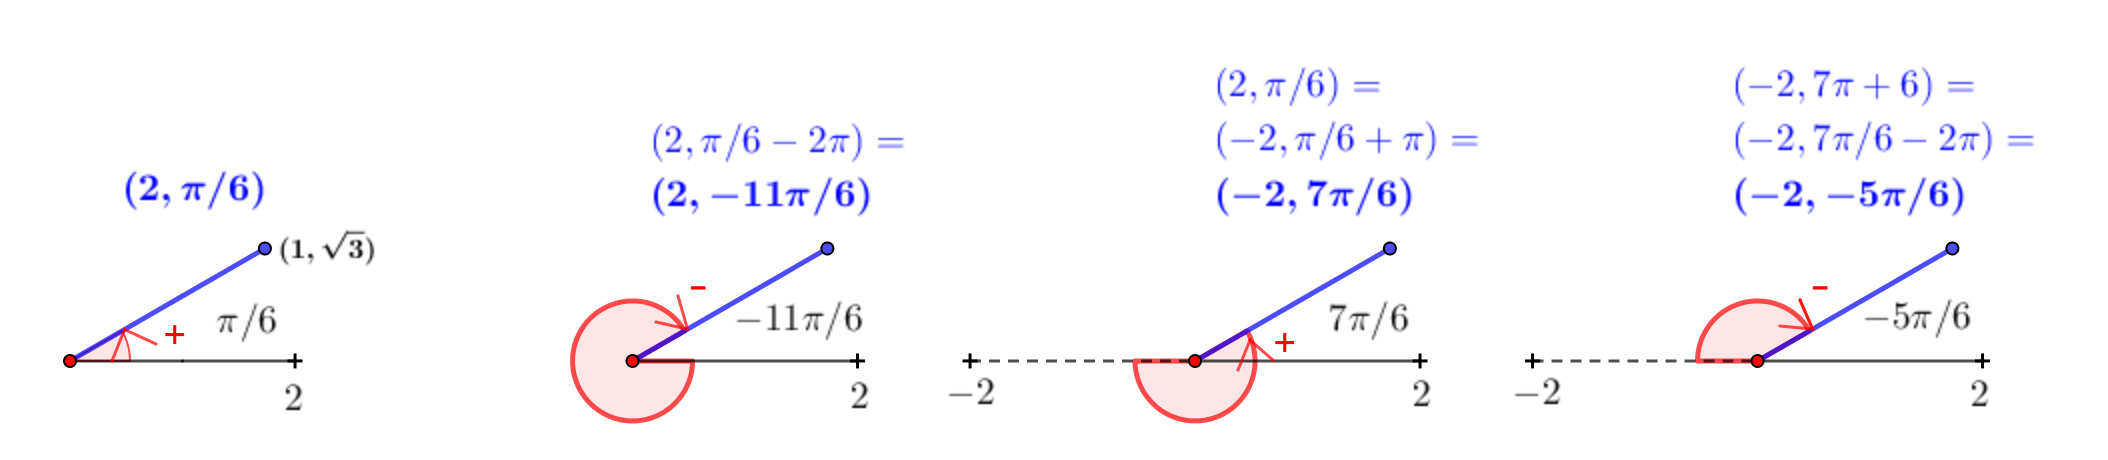
\includegraphics[width=.9\textwidth]{img-polares/polares24.png}
	\end{figure}

Mientras que en cartesianas las coordenadas de un punto $P(x,y)$ son únicas, en polares, debido a la imprecisión en el número de vueltas para la medida de ángulos, hay infinitas formas de dar un mismo punto $P(r,\theta+\boldsymbol{2k\pi}),\ \forall k\in \mathbb Z$

\begin{itemize}
\item 	Los puntos en que $r=a=cte, \ \forall \theta$ son circunferencias centradas en el origen o \emph{polo} de radio $r=a$.
\item   Los puntos para $\theta=\theta_0=cte,\ \forall r$ son semirrectas que pasan por el \emph{polo} y forman un ángulo $\theta=\theta_0$ con el eje polar.
\end{itemize}

\large{\textbf{Relación entre coordenadas polares y cartesianas}}\normalsize{:} Tomando el \emph{polo} como origen de coordenadas cartesianas y el eje $\mathcal OX+$ como el eje polar, tenemos:

\vspace{5mm}
\begin{cuadro-naranja}
\begin{multicols}{2}
	\begin{figure}[H]
	\centering
	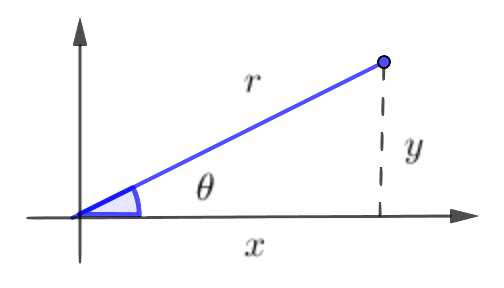
\includegraphics[width=.3\textwidth]{img-polares/polares22.png}
	\end{figure}
	%\textcolor{white}{$\quad$}
	\begin{equation*} \boxed{ \  \boldsymbol{
		\begin{cases} \ x=r\cos \theta \\ \ y=r\sin \theta \end{cases} \qquad 
		\begin{cases} \ r=\sqrt{x^2+y^2} \\ \ \tan \theta=\dfrac y x \end{cases}
		} \ }
	\end{equation*}
 \end{multicols}
\end{cuadro-naranja}

\vspace{10mm}

\begin{miejercicio}  

\hspace{1cm} a) Pasar a polares: $\ (1,1),\ (1,-1), \ (-\sqrt 3 , 1),\ (-5,0),\ (0,2)$; 

\hspace{1cm} b) Pasar a cartesianas:$\ (-2,\pi/3),\ (3,2\pi), (4,3\pi/2), (\sqrt 2, 5\pi/4)$

\rule{300pt}{0.2pt}

--- Cartesianas a polares:

$\triangleright \quad \boldsymbol{(1,1)} \quad x=1,\ y=1 \Rightarrow r=\sqrt{1^2+1^2}=\sqrt 2;\ \ \tan \theta=\dfrac{+1}{+1}\to \theta = \pi/4$

\hspace{5cm} $\boldsymbol{(1,1) \text{ cartesianas} \equiv (\sqrt 2, \pi/4) \text{ polares}}$

\begin{multicols}{2}
Las coordenadas polares no son unívocas: $\ (\sqrt 2,\pi/4)=(\sqrt 2, \pi/4+2k\pi), \ \forall k\in \mathbb Z$; además, si medimos la distancia negativa: $\ (\sqrt 2,\pi/4)=(-\sqrt 2,5\pi/4)=(-\sqrt 2,5\pi/4+2k\pi), \ \forall k\in \mathbb Z$
\begin{figure}[H]
	\centering
	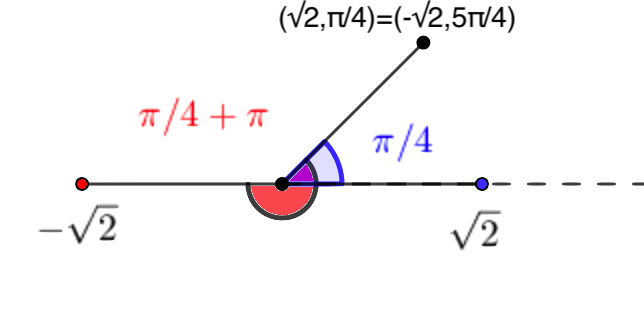
\includegraphics[width=.3\textwidth]{img-polares/polares23.png}
	\end{figure}
\end{multicols}

$\triangleright \quad \boldsymbol{(1,-1)} \quad x=1,\ y=-1 \Rightarrow r=\sqrt 2;\  \ \tan \theta=\dfrac{+1}{-1} \ \textcolor{gris}{ \to \mqty(\sin \theta < 0 \\ \cos \theta >0) \to } \ \theta = 7\pi/4$

\hspace{5cm} $\boldsymbol{(1,-1) \text{ cartesianas} \equiv (\sqrt 2, 7\pi/4) \text{ polares}}$

$\triangleright \quad \boldsymbol{(-\sqrt 3,1)} \quad x=-\sqrt 3,\ y=1 \Rightarrow r= $\scriptsize{ $\sqrt{(-\sqrt 3)^2+1^2}$ } \normalsize{$ =$}$2;\ \ \tan \theta=\dfrac{1}{-\sqrt 3} \textcolor{gris}{\footnotesize{\to \mqty(\sin + \\ \cos -) \to}} \ \theta = 5\pi/6$

\hspace{5cm} $\boldsymbol{(-\sqrt 3,1) \text{ cartesianas} \equiv ( 2, 5\pi/6) \text{ polares}}$

$\triangleright \quad \boldsymbol{(-5,0)}\quad x=5,\ y= 0 \Rightarrow r=5,\ \ \theta=\pi$ \small{Solo mirando la representación}\normalsize{.}

\hspace{5cm} $\boldsymbol{(-5,0) \text{ cartesianas} \equiv (5, \pi) \text{ polares}}$

$\triangleright \quad \boldsymbol{(0,2)} \quad x=0,\ y= 2 \, , \ $ \small{como en el caso anterior}\normalsize{:} $r=2;\ \ \theta=\pi/2$

\hspace{5cm} $\boldsymbol{(0,2) \text{ cartesianas} \equiv (2, \pi/2) \text{ polares}}$

--- Polares a cartesianas:

$\triangleright \quad \boldsymbol{(-2,\pi/3)}\quad r=-2,\ \theta = \pi/3 \ \leftrightarrow \ r=2,\ \theta=\pi/3+\pi=4\pi/3 \ \to \begin{cases} x=2\cos(5\pi/3)=-1\\ y=2\sin(5\pi/3)=-\sqrt 3 \end{cases}$ 

\hspace{5cm} $\boldsymbol{(-2,\pi/3) \text{ polares} \equiv (-1,-\sqrt 3) \text{ cartesianas}}$

$\triangleright \quad \boldsymbol{(3,2\pi)}=(3,0) \quad $\small{Solo mirando la representación}\normalsize{:}$\ (3,0)$

\hspace{5cm} $\boldsymbol{(3,2\pi) \text{ polares} \equiv (3,0) \text{ cartesianas}}$


$\triangleright \quad \boldsymbol{(4,3\pi/2)}\quad$ \small{Solo mirando la representación}\normalsize{:}$\ (0,-4)$

\hspace{5cm} $\boldsymbol{(4,3\pi/2) \text{ polares} \equiv (0,-4) \text{ cartesianas}}$

$\triangleright \quad \boldsymbol{(2,5\pi/4)}\quad \begin{cases} x=2\cos(5\pi/4)= -\sqrt 2 \\ y=2\sin(5\pi/4)=-\sqrt 2 \end{cases}$	

\hspace{5cm} $\boldsymbol{(2,5\pi/4) \text{ polares} \equiv (-\sqrt 2,-\sqrt 2) \text{ cartesianas}}$

\end{miejercicio}

\vspace{5mm}
\begin{miejercicio} 
	

Pasar a polares: $\ x^2+(y-3)^2=9$

 \rule{300pt}{0.2pt}

$r=x\cos \theta,\ y=r\sin \theta \ \to (r\cos \theta)^2+(r \sin \theta - 3)^2=9 \ \to \  r^2 - 6 r \sin \theta  \quad r\neq 0  \ \to$

\hspace{5cm} $\boldsymbol{r=6\sin \theta}$
\end{miejercicio}

\vspace{5mm}
\begin{miejercicio} 
	

 Pasar a cartesianas: 

\hspace{2.6cm} $a) \ \  r\cos \theta =4 \ ; \qquad b)\ \   r^2=4r\cos \theta\ ; \qquad c)\ \   r=\dfrac 4{2\cos \theta - \sin \theta}$

 \rule{300pt}{0.2pt}

$\triangleright \ \ a)\quad  r\cos \theta = 4 \quad \Rightarrow  \boldsymbol{x=4}\ $ Recta vertical.

$\triangleright \ \ b)\quad   r^2=4r\cos \theta\ \Rightarrow x^2+y^2=4 x \to x^2-4x+\textcolor{red}{4} + y^2= \textcolor{red}{4} \to \boldsymbol{(x-2)^2+y^2=2^2} \ $ 
Circunferencia de centro $(2,0)$ y radio $2$.

$\triangleright \ \ c)\quad  r=\dfrac 4{2\cos \theta - \sin \theta} \to 2r\cos \theta -r\sin \theta = 4 \quad \Rightarrow  2x-y=4 \to \boldsymbol{y=2x-4} \ $ Recta de pendiente $2$ y ordenada en el origen $-4$.
\end{miejercicio}


\vspace{5mm}
\begin{mipropuesto} 

\begin{multicols}{2}
Pasar a polares:

$\quad a)\quad x^2+y^2=4$

$\quad b)\quad x=y$

$\quad c)\quad x^2+(y-2)^2=4$	

$\quad d)\quad x^2+xy+y^2=1$

Paras a cartesianas:

$\quad e)\quad r=4\cosec \theta$

$\quad f)\quad r^2\sin 2\theta=2$

$\quad g)\quad \cos^2 \theta = \sin^2 \theta$

$\quad h)\quad r=2\cos \theta-\sin \theta$
\end{multicols}
	
\end{mipropuesto}

$\triangleright \ \ a)\ \ x^2+y^2=4 \to (r\cos \theta)^2+(r\sin \theta)^2=4 \to \boldsymbol{r^2=4}$

$\triangleright \ \ b)\ \ x=y \to r\cos \theta=r\sin \theta \to \tan \theta=1 \to \boldsymbol{\theta =\pi/4 \ \ \wedge \ \ \theta = 5\pi/4}$

$\triangleright \ \ c)\ \ x^2+(y-2)^2=4 \to (r\cos \theta)^2+(r\sin \theta-2)^2=4 \to r^2-4r\sin \theta + 4=4 \to \boldsymbol{r=4\sin \theta}$

$\triangleright \ \ d)\ \ x^2+xy+y^2=1 \to (r\cos \theta)^2+(r\cos \theta r \sin \theta)+(r\sin \theta )^2=1 \to \boldsymbol{ r^2(1+\sin \theta \cos \theta )=1}$

$\triangleright \ \ e)\ \ r=4\cosec \theta \to r\sin \theta=4 \to \boldsymbol{y=4}$

$\triangleright \ \ f)\ \ r^2\sin 2\theta = 2 \to 2r\cos\theta \ r\sin \theta=2 \to 2xy=2 \to \boldsymbol{xy=1}$

$\triangleright \ \ g)\ \ \cos^2 \theta=\sin^2\theta \to r^2\cos^2 \theta=r^2\sin^2\theta \to |x|=|y| \to \boldsymbol{y=x \ \ \wedge \ \ y=-x}$ 

$\triangleright \ \ h)\ \ r=2\cos\theta -\sin \theta \to r^2=2r\cos\theta -r\sin \theta \to x^2+y^2=2x-y \to x^2-2x+y^2+y=0 \to x^2-2x\textcolor{red}{+1-1}+y^2+y+\textcolor{red}{+1/4-1/4}=0 \to (x-1)^2-1+(y+1/2)^2-1/4=0 \to \boldsymbol{(x-1)^2+(y+1/2)^2=5/4}$

\begin{flushright}\textcolor{teal}{\rule{250pt}{0.2pt}}	\end{flushright}


\section{Gráficas en coordenadas polares}

\vspace{-5mm}

\begin{tikzpicture}
	\fill [left color=red!50, right color=teal!50] (0,0) rectangle (3.5,.1);
	\fill [left color=teal!50, right color=blue!50] (3.5,0) rectangle (7.5,.1);
	\end{tikzpicture}
\vspace{0.5cm}

Para representar una curva polar, $r=r(\theta)$, usaremos el sistema de referencia polar: ``circunferencias concéntricas centradas en el polo y rayos que salen del polo a ángulos conocidos	''. \textcolor{gris}{(Otro modo de hacerlo es construir una tabla $\theta|r$, pasar a cartesianas $x|y$ y representar en un sistema de referencia cartesiano)}.

\vspace{5mm}

\begin{miejercicio} 
	
Representa la curva polar: $\ r=2\sin \theta$

 \rule{300pt}{0.2pt}


\begin{table}[H]
\centering
\begin{tabular}{c|ccccccccc}
$\boldsymbol{r}$ & $0$ & $\pi/6$ & $\pi/4$  & $\pi/3$ & $\pi/2$ & $2\pi/3$ & $3\pi/4$ & $5\pi/6$ & $\pi$ \\ \hline
$\boldsymbol{\theta}$ & $0$ & $1$ & $\sqrt 2$ & $\sqrt 3$ & $2$ & $\sqrt 3$ & $\sqrt 2$ & $1$ & $0$
\end{tabular}
\end{table}

\begin{multicols}{2}
Para $\pi<\theta<2\pi$ los valores se repiten dando $r<0$, por ejemplo:

$\theta=3\pi/2 \to r=2\sin (2\cdot 3\pi/2)=2\sin(3\pi)=2\sin(\pi)=2(-1)=-2$

Pero, $(-2,3\pi/2)=)(2,3\pi/2+\pi)=(2,\pi/2)$
\begin{figure}[H]
	\centering
	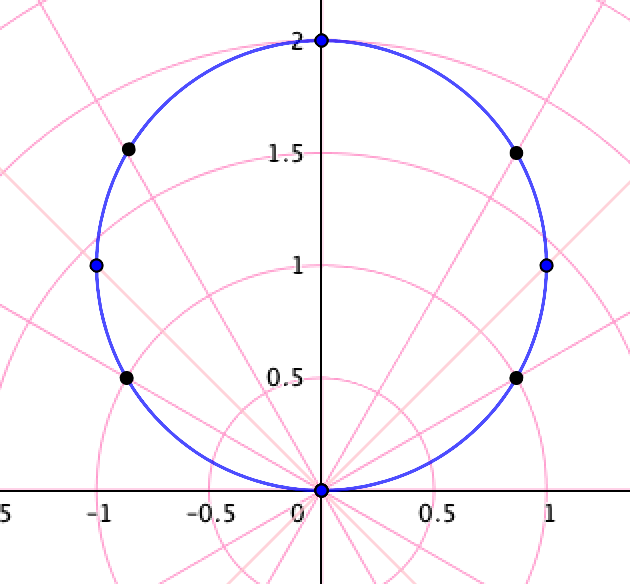
\includegraphics[width=.3\textwidth]{img-polares/polares25.png}
\end{figure}	
\end{multicols}
\end{miejercicio}

\underline{Observaciones}: \tiny{$\qquad \blacksquare \quad $}\normalsize{En} general, las curvas $\ r=2a \sin \theta\, ;\ \ r=2a\cos \theta \ $ son \emph{circunferencias} de radio $r=|a|$ centradas en $(a,\pi/2)$ y en $(a,0)$, respectivamente.



\vspace{5mm}

\begin{mipropuesto}

Representa $\ \ r=2+2\cos \theta$
\end{mipropuesto}
\begin{table}[H]
\centering
\begin{tabular}{c|ccccccccc}
$\boldsymbol{r}$ & $0$ & $\pi/4$ & $\pi/2$ & $3\pi/4$ & $\pi$ & $5\pi/4$ & $3\pi/2$ & $7\pi/4$ &  $2\pi$\\ \hline
$\boldsymbol{\theta}$ & $4$ & $2+\sqrt 2$ & $2$ & $2-\sqrt 2$ & $0$ & $2-\sqrt 2$ & $2$ & $12+\sqrt 2$ & $4$
\end{tabular}
\end{table}

\begin{multicols}{2}

\underline{Observaciones}: 
\tiny{$\qquad \blacksquare \quad $}\normalsize{En} general, 


\hspace{10mm}$r=a(1\pm \sin \theta)\, ; \ \ r=a(1\pm \cos \theta)\ $ 

\hspace{10mm}son \emph{cardioides}.

\textcolor{gris}{$f(-\theta)=f(\theta)$}, simetria respecto del eje polar (ver más adelante).
\begin{figure}[H]
	\centering
	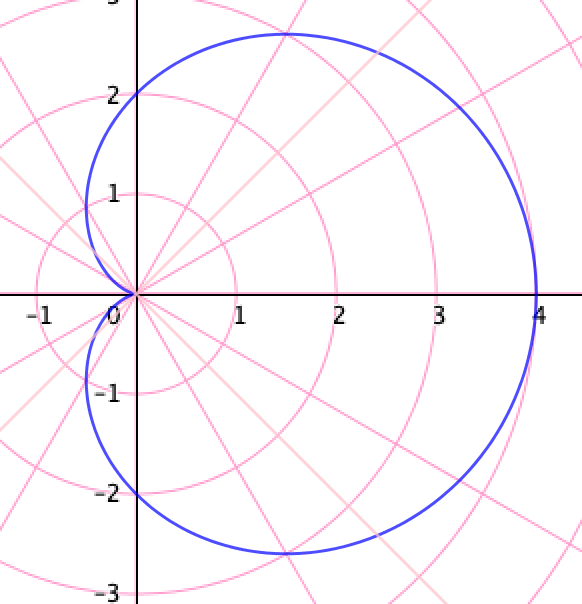
\includegraphics[width=.25\textwidth]{img-polares/polares26.png}
\end{figure}
\end{multicols}

\vspace{5mm}
\begin{mipropuesto}

Representa $\ \ r=6+3\cos \theta$
\end{mipropuesto}

\begin{multicols}{2}

\underline{Observaciones}: 
\tiny{$\qquad \blacksquare \quad $}\normalsize{En} general, 


\hspace{10mm}$r=a \pm b \cos \theta \, ; \ \ r=a \pm b \sin \theta\, , \ \ |a|>|b| $ 

\hspace{10mm}son \emph{limaçon} o caracoles (sin rizo).


\begin{figure}[H]
	\centering
	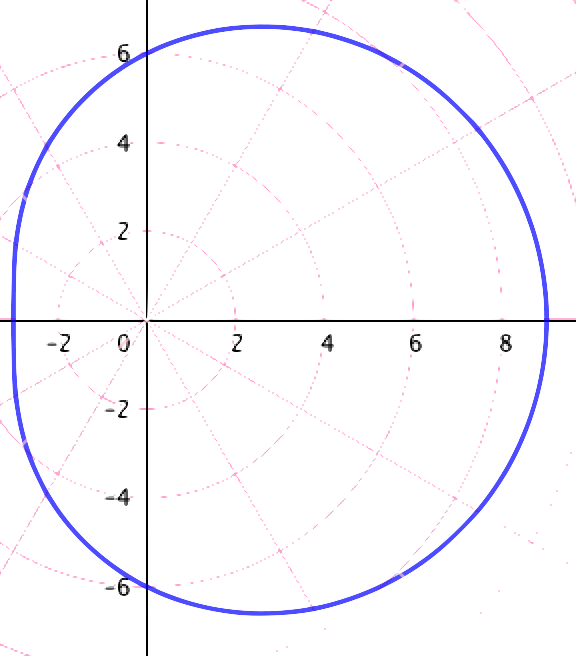
\includegraphics[width=.2\textwidth]{img-polares/polares48.png}
\end{figure}
\end{multicols}


\vspace{5mm}
\begin{mipropuesto}

Representa $\ \ r=3+6\cos \theta$
\end{mipropuesto}

\begin{multicols}{2}

\underline{Observaciones}: 
\tiny{$\qquad \blacksquare \quad $}\normalsize{En} general, 



\hspace{10mm}$r=a \pm b \cos \theta \, ; \ \ r=a \pm b \sin \theta\, , \ \ |a|<|b| $ 

\hspace{10mm}son \emph{limaçon} o caracoles (con rizo).


\begin{figure}[H]
	\centering
	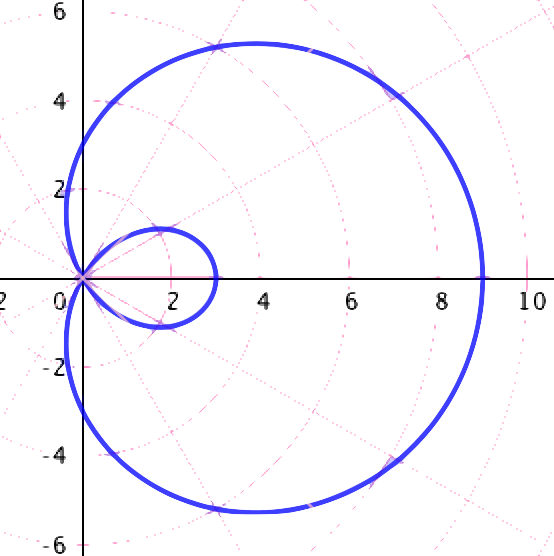
\includegraphics[width=.2\textwidth]{img-polares/polares49.png}
\end{figure}
\end{multicols}

\vspace{5mm}

\begin{mipropuesto}

Representa $\ \ r=\cos 2\theta$
\end{mipropuesto}

\begin{table}[H]
\centering
\begin{tabular}{c|ccccccccc}
$\boldsymbol{r}$ & $0$ & $\pi/6$ & $\pi/4$  & $\pi/3$ & $\pi/2$ & $2\pi/3$ & $3\pi/4$ & $5\pi/6$ & $\pi$ \\ \hline
$\boldsymbol{\theta}$ & $1$ & $1/2$ & $0$ & $-1/2$ & $-1$ & $-1/2$ & $0$ & $1/2$ & $1$
\end{tabular}
\end{table}

\begin{multicols}{2}
\underline{Observaciones}: 
\tiny{$\qquad \blacksquare \quad $}\normalsize{En} general, 

\hspace{10mm}$r=a \cos n \theta\, ; \ \ r=a  \sin n \theta\ $ 

\hspace{10mm} son \emph{rosas}. 

\hspace{10mm} de $n$ pétalos si $n$ es impar 

\hspace{10mm} o de $2n$ pétalos i $n$ par.	

\begin{figure}[H]
	\centering
	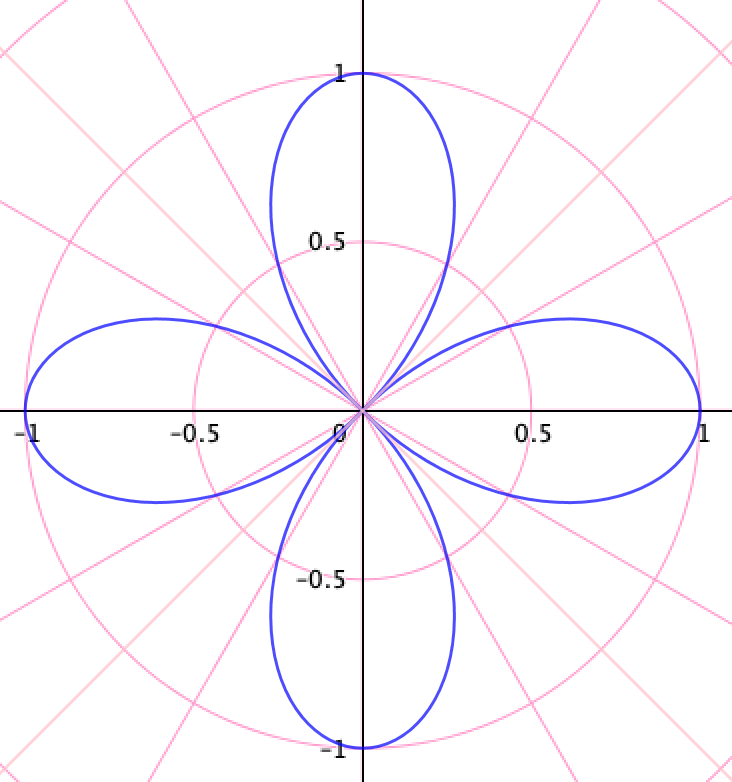
\includegraphics[width=.25\textwidth]{img-polares/polares27.png}
\end{figure}
\end{multicols}


\vspace{5mm}
\begin{mipropuesto}

Representa $\ \ r^2=4\cos 2\theta$
\end{mipropuesto}

\begin{multicols}{2}

\underline{Observaciones}: 
\tiny{$\qquad \blacksquare \quad $}\normalsize{En} general, 



\hspace{10mm}$r^2=a \cos 2\theta \, ; \ \ r^2=a \sin 2\theta\, , \ \ |a|<|b| $ 

\hspace{10mm}son \emph{lemniscatas}.


\begin{figure}[H]
	\centering
	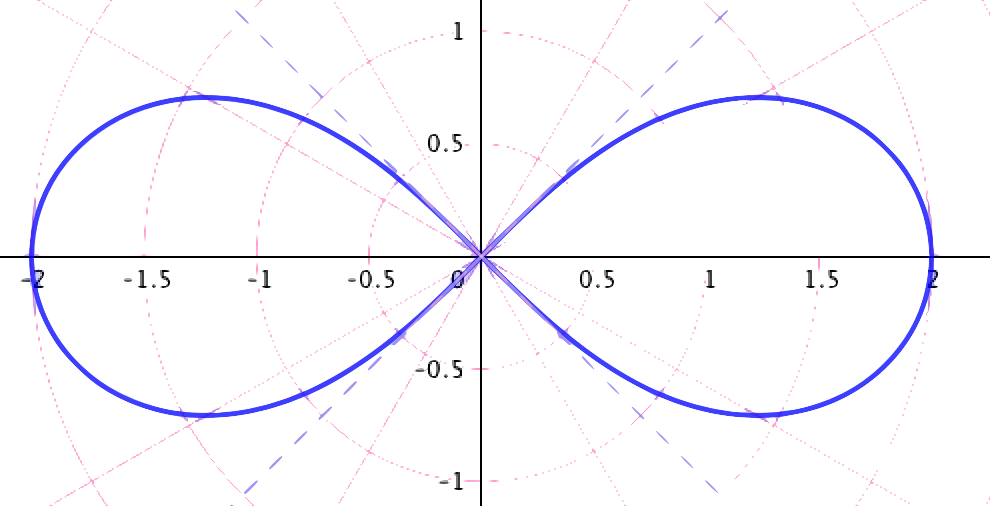
\includegraphics[width=.3\textwidth]{img-polares/polares50.png}
\end{figure}
\end{multicols}

\vspace{5mm}
\begin{mipropuesto}

Representa $\ \ r=2\theta\, ; \qquad r=2e^{0.3\theta}$
\end{mipropuesto}


\underline{Observaciones}: 
\tiny{$\qquad \blacksquare \quad $}\normalsize{En} general, 

\hspace{10mm}$r^2=a \theta \ $ son \emph{espirales de Arquímedes}.
$\qquad \qquad$
\hspace{10mm}$r^2=a e^{b \theta} \ $ son \emph{espirales logarítmicas}.

\begin{multicols}{2}
\begin{figure}[H]
	\centering
	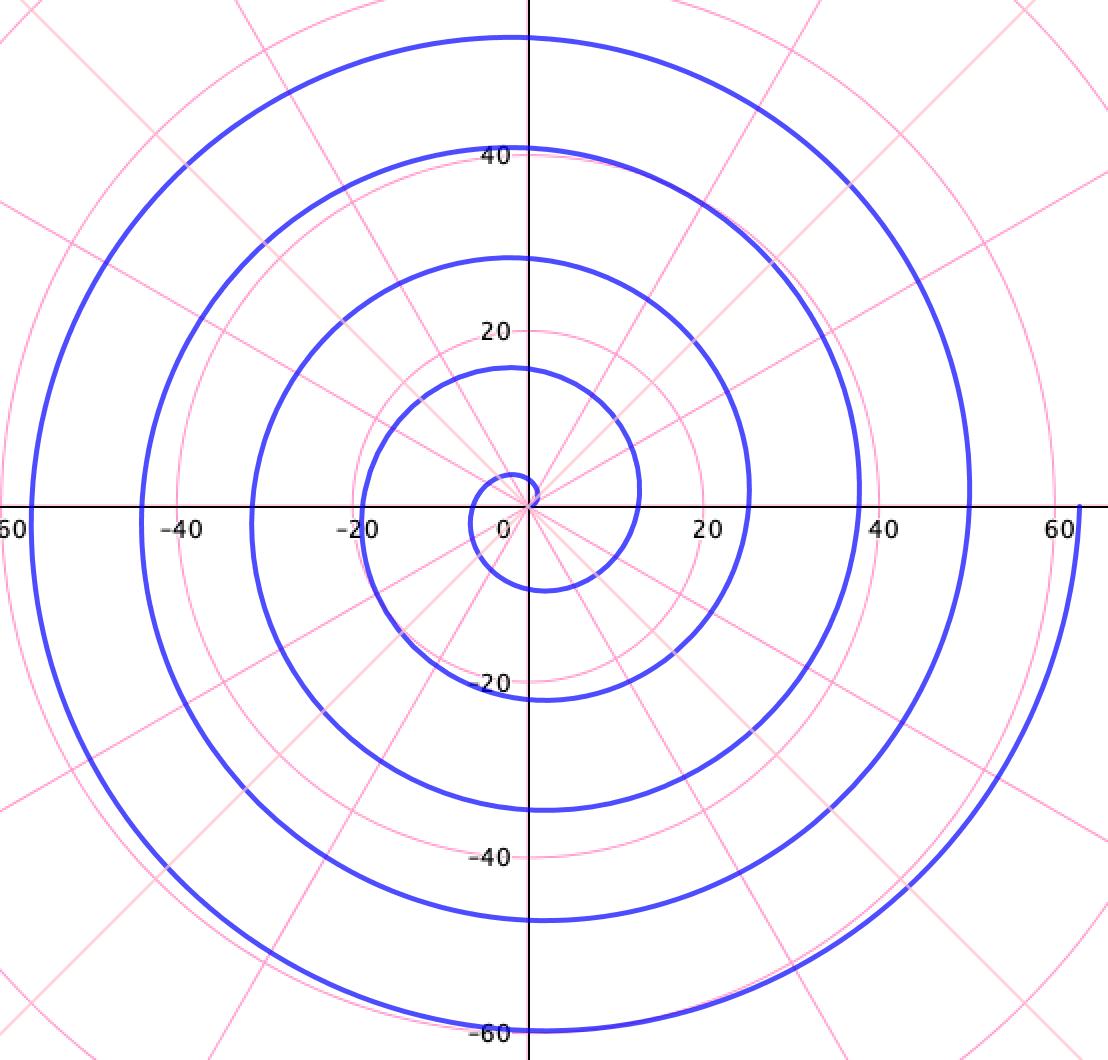
\includegraphics[width=.3\textwidth]{img-polares/polares51.png}
\end{figure}
\begin{figure}[H]
	\centering
	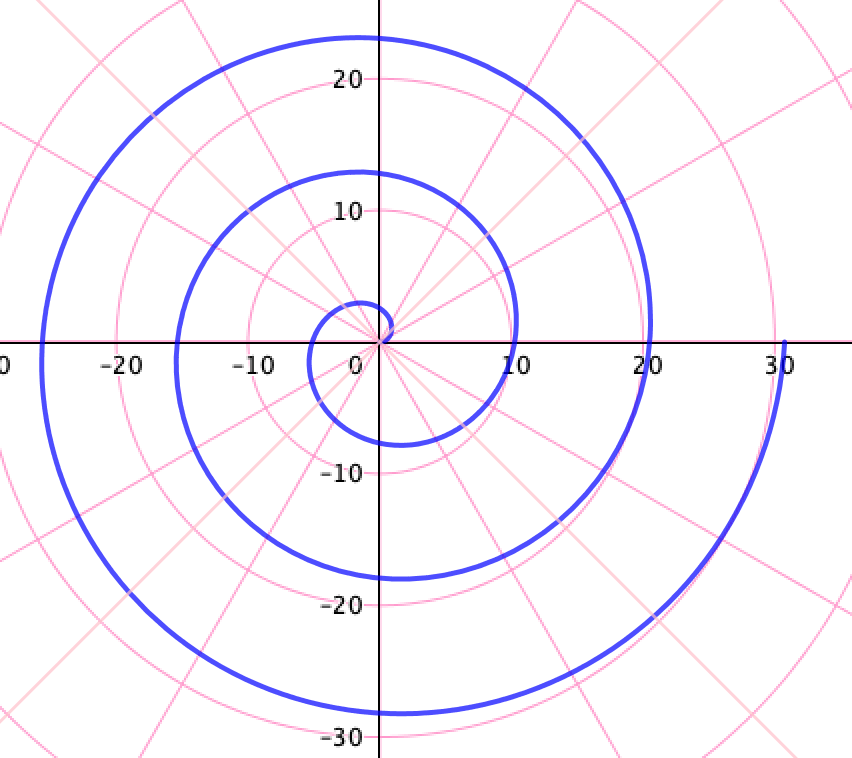
\includegraphics[width=.3\textwidth]{img-polares/polares52.png}
\end{figure}
\end{multicols}

\begin{flushright}\textcolor{teal}{\rule{250pt}{0.2pt}}	\end{flushright}	

%\color{ForestGreen}
\color{teal}
\rule{250pt}{0.2pt}

\begin{small}
Una espiral logarítmica, espiral equiangular o espiral de crecimiento es la curva definida por un objeto que se mueve con velocidad lineal constante y velocidad angular.

La característica fundamental de esta espiral es que la expansión y la rotación tienen un vínculo geométrico o exponencial. La distancia entre las espiras aumenta mucho más rápidamente que la rotación.

Otros nombres que recibe esta espiral es la de equiangular o geométrica; el primer nombre lo recibe ya que el mismo ángulo de giro, puestos a construirla, crece en progresión aritmética, mientras que el segundo nombre lo recibe por el radio que crece en progresión geométrica.

Este espiral es el que mas podemos observar en la naturaleza, en el reino vegetal, en las formas de las galaxias, en las conchas de algunas especies de moluscos, etc. Es también usado en el arte desde épocas prehistóricas\end{small}\normalsize{.}
	
\begin{figure}[H]
	\centering
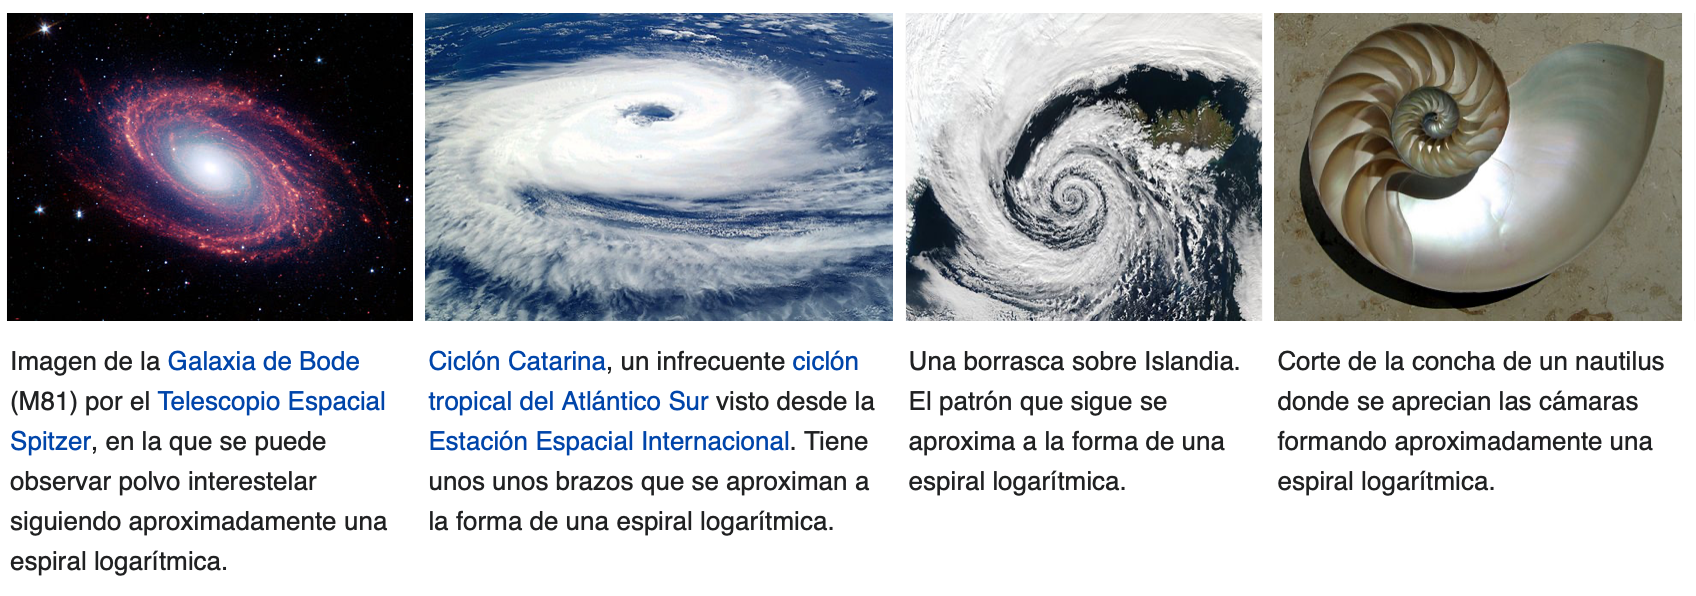
\includegraphics[width=.95\textwidth]{img-polares/polares53.png}
\end{figure}

\vspace{-15mm}
\begin{flushright}
\rule{250pt}{0.2pt}		
\end{flushright}

\color{black}
\vspace{5mm}
\large{Otras curvas en polares}\normalsize{.}
	
	
\begin{figure}[H]
	\centering
	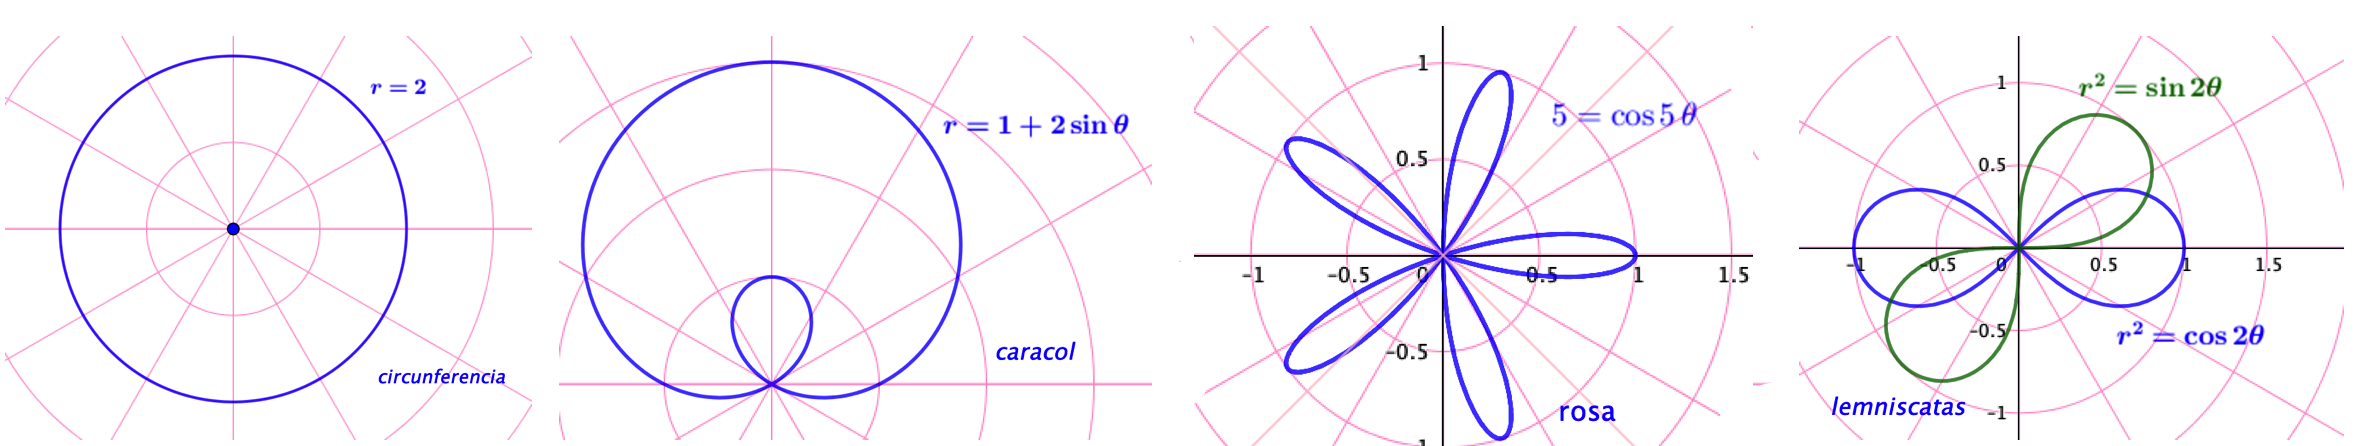
\includegraphics[width=1\textwidth]{img-polares/polares29.png}
\end{figure}

\vspace{5mm}	
\begin{multicols}{2}
$\quad$ 

Para curvas complicadas es conveniente usar un sw. adecuado.

Se incluye, con estos apuntes, el applet de \emph{geogebra} \textsf{`polares01.ggb'}.	

\begin{figure}[H]
	\centering
	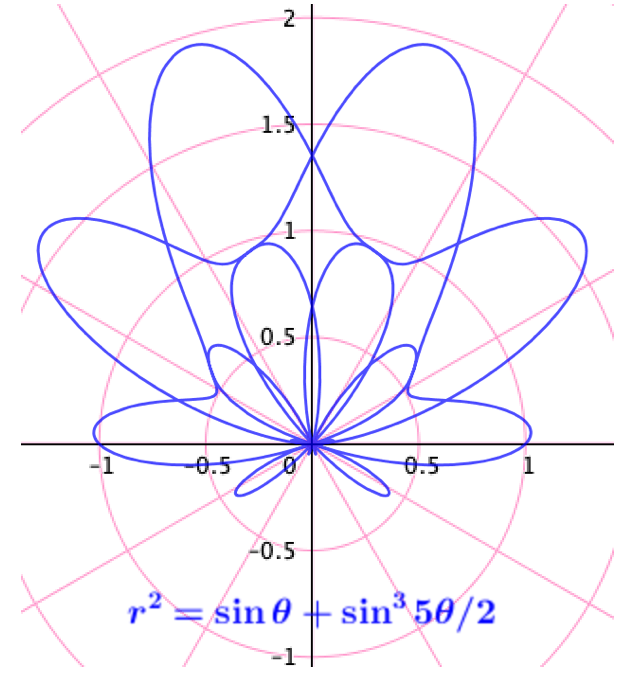
\includegraphics[width=.25\textwidth]{img-polares/polares30.png}
\end{figure}
\end{multicols}

\vspace{5mm}
\textbf{\large{Simetrías}}\normalsize{:}
	
	En ocasiones, el estudio de la simetría de una curva simplifica el estudio de su representación.
\vspace{-5mm}	
\begin{itemize}
\item Si la ecuación de la curva no varía al cambiar $\theta$ por $-\theta$,	 entonces la curva es \emph{simétrica respecto del eje polar.}
\item Si la ecuación de la curva no varía al cambiar $r$ por $-r$,	 entonces la curva es \emph{simétrica respecto al polo.}
\item Si la ecuación de la curva no varía al cambiar $\theta$ por $\pi-\theta$,	 entonces la curva es \emph{simétrica respecto al rayo $\theta=\pi/2$ \textcolor{gris}{(eje $y$)}.}
\end{itemize}

	
\begin{figure}[H]
	\centering
	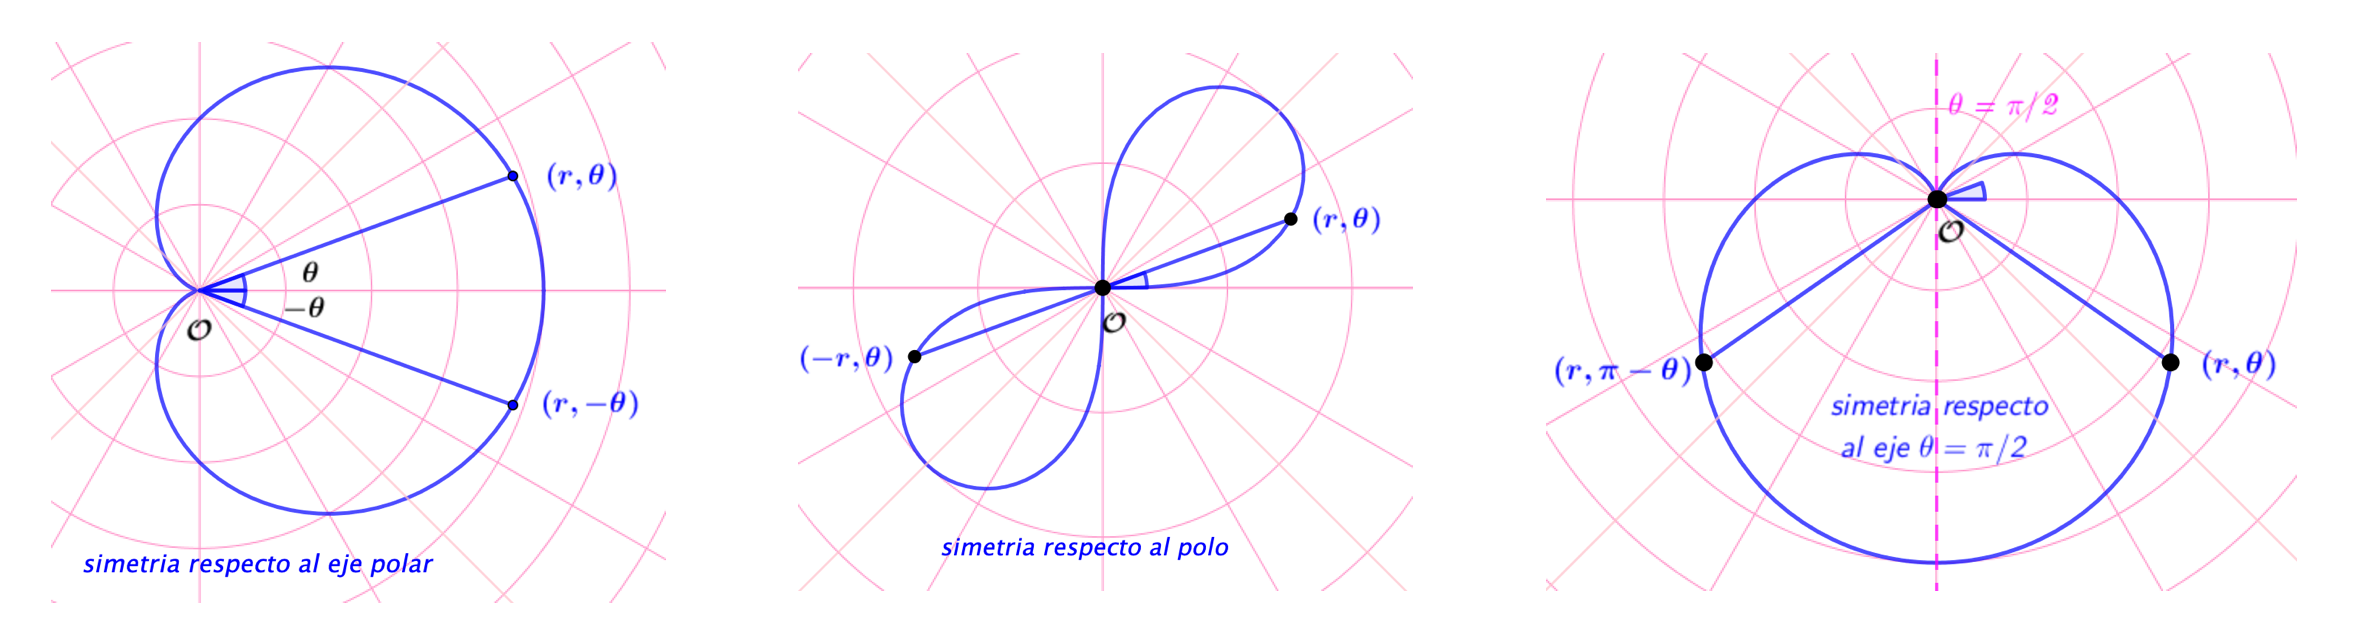
\includegraphics[width=1\textwidth]{img-polares/polares28.png}
\end{figure}


	

\section{Rectas y circunferencias en polares}

\vspace{-5mm}

\begin{tikzpicture}
	\fill [left color=red!50, right color=teal!50] (0,0) rectangle (3.5,.1);
	\fill [left color=teal!50, right color=blue!50] (3.5,0) rectangle (7.5,.1);
	\end{tikzpicture}
\vspace{0.5cm}
	


\subsection{Rectas}
\vspace{-5mm}

\begin{tikzpicture}
	\fill [left color=red!50, right color=teal!50] (0,0) rectangle (3.5,.01);
	\fill [left color=teal!50, right color=blue!50] (3.5,0) rectangle (7.5,.01);
	\end{tikzpicture}

\begin{multicols}{2}
$\triangleright \ \ $ Si la recta contiene al polo (pasa por él) tenemos, en cartesianas, una ecuación del tipo $\ y=mx \ $ con $ \ m=\tan \theta_0)$. pasando a polares, \textcolor{gris}{$(x=r\cos \theta\, , \ y=r\sin \theta)$}: $\ y=mx \to   r\sin \theta = m r \cos \theta \to \tan \theta=m=\tan \theta_0 \ \to \qquad  \boxed{ \ \subrayado{\theta=\theta_0} \ }\quad $ Recta, en forma polar, que pasa por el polo con ángulo $\theta_0$.
\begin{figure}[H]
	\centering
	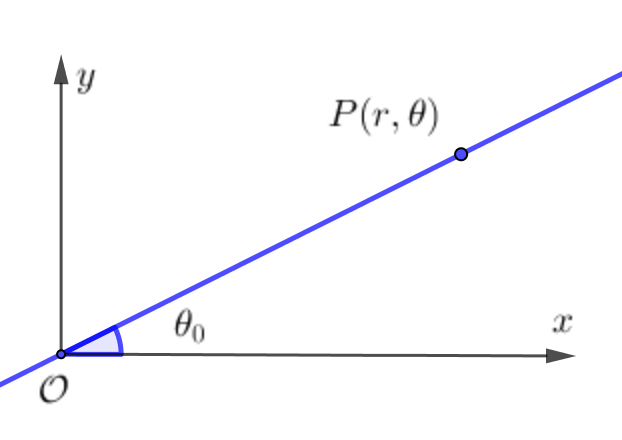
\includegraphics[width=.3\textwidth]{img-polares/polares40.png}
\end{figure}
\end{multicols}


\begin{multicols}{2}
$\triangleright \ \ $ Sea $P_0(r_0,\theta_0)$ la proyección ortogonal del polo $\mathcal O$ sobre la recta $R$, con ello, la ecuación de $R$ es:

$$ \boxed{ \ \subrayado{ \ r\cos (\theta-\theta_0)=r_0 \ } \ } \quad \to \ \quad r=\dfrac{r_0}{\cos (\theta-\theta_0)}$$

Recta que no contiene al polo, está a distancia $r_0$ de éste y su perpendicular forma un ángulo $\theta_0$ con el eje polar.

\begin{figure}[H]
	\centering
	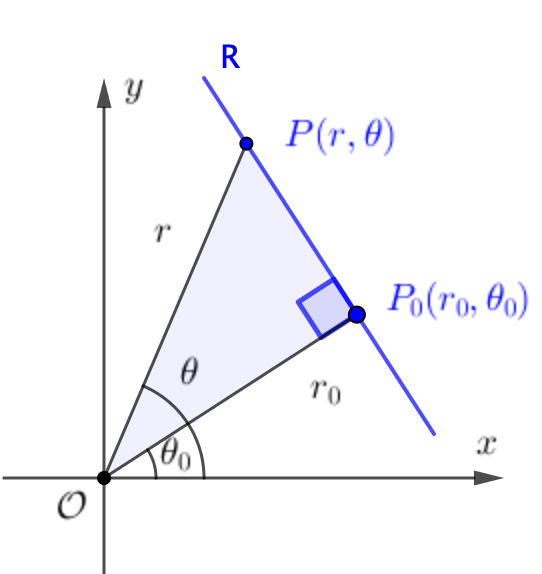
\includegraphics[width=.3\textwidth]{img-polares/polares35.png}
\end{figure}	
\end{multicols}

\underline{Observaciones}:
\vspace{-5mm}

\begin{itemize}
\item $\theta_0=0 \ \ \ \to \ \ \, r=\dfrac {r_0}{\cos \theta} \quad $ es una recta vertical.	
$\qquad \ \ \, $ \textcolor{gris}{Para $\ \theta_0=\pi \ \to \ r=-\dfrac d {\cos \theta}$}
\item $\theta_0=\pi/2 \ \to \ r=\dfrac {r_0}{\sin \theta} \quad $ es una recta horizontal. 
$\qquad$ \textcolor{gris}{Para $\ \theta_0=3\pi/2 \ \to \ r=-\dfrac d {\sin \theta}$}.
\end{itemize}

\vspace{-5mm}
\begin{figure}[H]
	\centering
	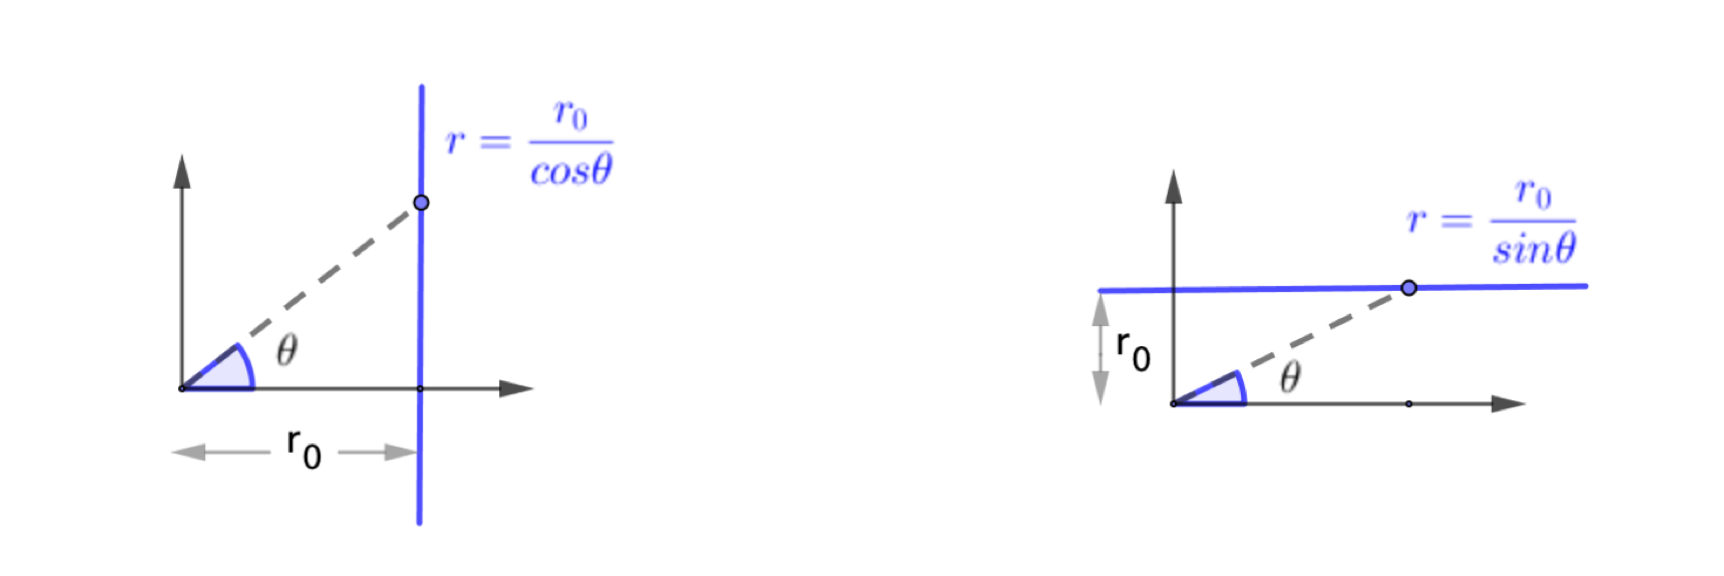
\includegraphics[width=.75\textwidth]{img-polares/polares41.png}
\end{figure}


\begin{miejercicio} 
	

Recta $\  \theta_0=\pi/3;\ \ r_0=2$ 

\rule{300pt}{0.2pt}

\begin{multicols}{2}
$\qquad \boldsymbol{ r\cos (\theta-\pi/3)=2}$ 

$\qquad r(\cos \theta \cos \pi/3 + \sin \theta \sin \pi/3)=2$ 

$\qquad \frac 1 2 r \cos \theta + \frac {\sqrt 3}2 \sin \theta = 2$

$\qquad \boldsymbol{x+\sqrt 3 y=4}$
\begin{figure}[H]
	\centering
	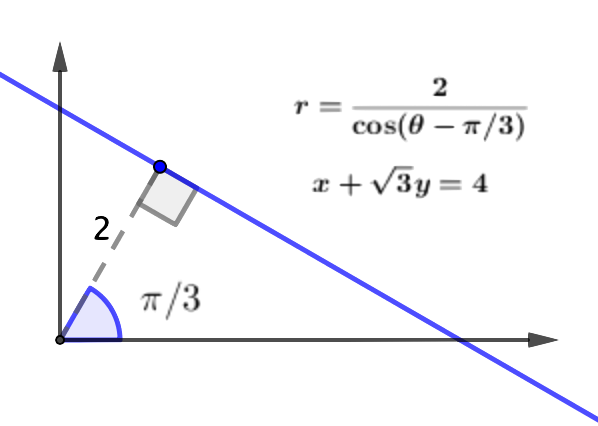
\includegraphics[width=.35\textwidth]{img-polares/polares42.png}
\end{figure}
\end{multicols}

\end{miejercicio}

\vspace{5mm}	
\subsection{Circunferencias}
\vspace{-5mm}

\begin{tikzpicture}
	\fill [left color=red!50, right color=teal!50] (0,0) rectangle (3.5,.01);
	\fill [left color=teal!50, right color=blue!50] (3.5,0) rectangle (7.5,.01);
	\end{tikzpicture}


$\triangleright \ \ $ Circunferencia con centro en el polo $\mathcal O$  y radio  $a$: 

En cartesianas: $ \ x^2+y^2=a^2 \ \to \ $ pasando a polares: $ \ (r \cos \theta)^2+(r \sin \theta)^2=a^2 \, , \ $

puesto que $\sin^2 \theta+\cos^2 \theta=1\, , \  $ se tiene:
$ \qquad \boxed{ \ \subrayado { \ \boldsymbol{r=a} \ } \ }$


\begin{multicols}{2}
\textcolor{white}{.}

$\triangleright \ \ $ Circunferencia de radio $\ a \ $ y centro en $\ P_0(r_0,\theta_0)\, $ 

por la ley de cosenos al $\mathcal O P_0 P\, :$

$$ \boxed{ \ \subrayado{ \ a^2 \ =\  r^2\, +\, r_0^2\, -\, 2\, r\, r_0\,  \cos (\theta-\theta_0) \ } \ }$$

\textcolor{white}{.}
\begin{figure}[H]
	\centering
	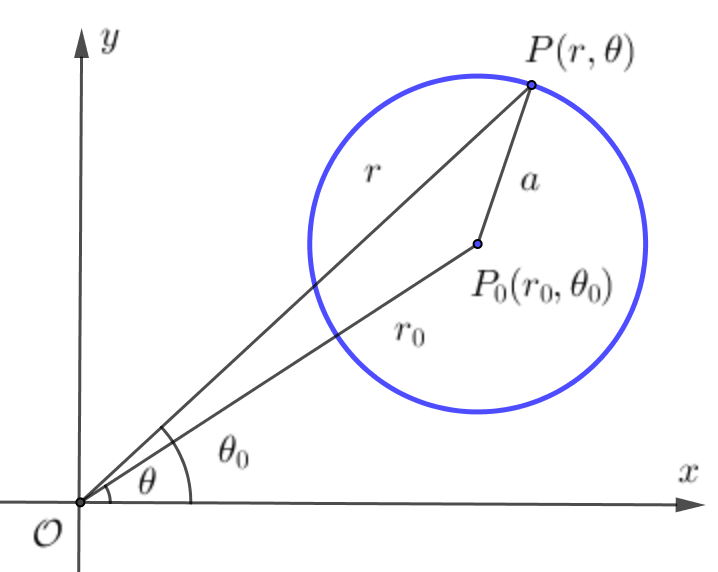
\includegraphics[width=.3\textwidth]{img-polares/polares36.png}
\end{figure}	
\end{multicols}


\underline{Observaciones}:
\vspace{-3mm}
\begin{itemize}
\item Si la circunferencia pasa por el origen: $\ r_0=a \ \to \ a^2=a^2+r^2-2ra\cos (\theta-\theta_0) \ \to $
 
$\to \ r^2=2ra\cos (\theta-\theta_0) \ \to \ \boldsymbol {r=2a \cos (\theta-\theta_0) } $
\item 	Si el centro está en $\mathcal OX+ \ \ \theta_0 = 0 \ \boldsymbol{r=2a \cos \theta}\, ; \quad $ si el centro está en $\mathcal OX- \ \ \theta_0 = 0 \ \boldsymbol{r=-2a \cos \theta}$
\item Si el centro está en $\mathcal OY+ \ \ \theta_0 = 0 \ \boldsymbol{r=2a \sin \theta}\, ; \quad $ si el centro está en $\mathcal OY- \ \ \theta_0 = 0 \ \boldsymbol{r=-2a \sin \theta}$
\end{itemize}


\begin{miejercicio} 
	

 Graficar $\  r=4\cos (\theta-\pi/3)$ 

 \rule{300pt}{0.2pt}

\begin{multicols}{2}
Por inspección de la ecuación 

\textcolor{gris}{$\ (r=2a \cos (\theta-\theta_0) \ $) }

concluimos que se trata de una circunferencia que pasa por el polo, de radio 2 y con centro en $(2,\pi/3)$.
\begin{figure}[H]
	\centering
	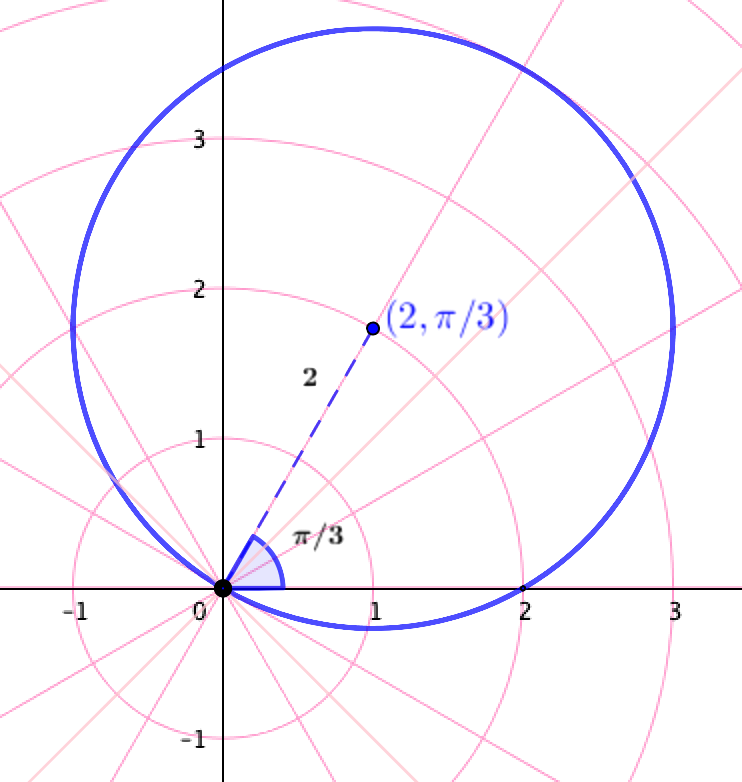
\includegraphics[width=.25\textwidth]{img-polares/polares43.png}
\end{figure}
\vspace{2mm}
\end{multicols}

\end{miejercicio}




\vspace{5mm}
\section{Cálculo en polares}

\vspace{-5mm}

\begin{tikzpicture}
	\fill [left color=red!50, right color=teal!50] (0,0) rectangle (3.5,.1);
	\fill [left color=teal!50, right color=blue!50] (3.5,0) rectangle (7.5,.1);
	\end{tikzpicture}
\vspace{0.5cm}


\vspace{5mm}

\large{\textbf{Distancia entre dos puntos}}\normalsize{:}

\begin{multicols}{2}

Por el teorema del coseno, 

\begin{adjustwidth}{30pt}{25pt}
\begin{destacado}
$  d\, (\, (r_1,\theta_1),(r_2,\theta_2)\, ) =  \\ \\\sqrt{r_1^2+r_2^2-2r_1r_2\cos(\theta_2-\theta_1)} $	
\end{destacado}
\end{adjustwidth}

\begin{figure}[H]
	\centering
	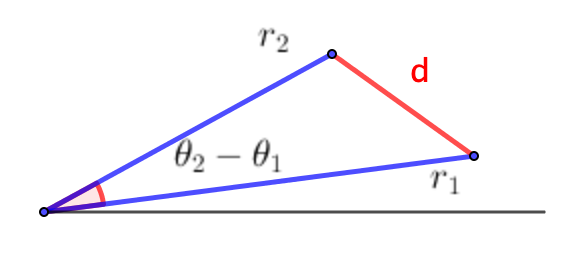
\includegraphics[width=.35\textwidth]{img-polares/polares31.png}
\end{figure}

\end{multicols}


\vspace{5mm}

\large{\textbf{Recta tangente}}\normalsize{:}

\vspace{5mm}

Parametrizando la curva,

$r=f(\theta) \to \begin{cases} 
 \ x=r\cos \theta = f(\theta)\cos \theta & \to \displaystyle \dv{x}{\theta}= f'(\theta)\cos \theta - f(\theta)\sin \theta	 \\ \\ 
 \ y=r\sin \theta = f(\theta)\sin \theta & \to \displaystyle \dv{y}{\theta}= f'(\theta)\sin \theta + f(\theta)\cos \theta
 \end{cases}$
 
 La pendiente de la recta tangente es:
 
 $$\boxed{ \ \subrayado{ \ 
 \displaystyle \eval{\dv{x}{y}}_{(r,\theta)}= \dfrac{f'(\theta)\sin \theta + f(\theta)\cos \theta}{f'(\theta)\cos \theta - f(\theta)\sin \theta}
 \ } \ }$$



\vspace{5mm}

\large{\textbf{Área bajo una curva}}\normalsize{:}

%\vspace{5mm}

\begin{multicols}{2}

$\quad$

$\qquad \boxed{ \ \subrayado{ \ A\ = \ \displaystyle \int_{\theta_1}^{\theta_2} \dfrac 1 2 \, r^2\, \dd \theta \ = \int_{\theta_1}^{\theta_2} \dfrac 1 2 \, f(\theta)^2\, \dd \theta  \ } \ }$

\begin{figure}[H]
	\centering
	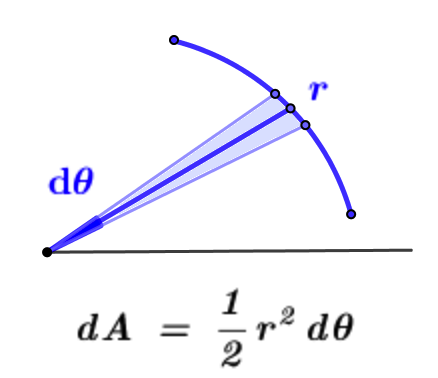
\includegraphics[width=.25\textwidth]{img-polares/polares32.png}
\end{figure}

\end{multicols}




\vspace{5mm}

\begin{miejercicio} 

Calcular el área encerrada por el cardioide $ r=2(1+\cos\theta)\ $ en $[0,2\pi]$.

\rule{300pt}{0.2pt}

$A=\displaystyle \int_0^{2\pi} \dfrac 1 2 \, 4\, (1+\cos \theta)^2\, \dd \theta =\int_0^{2\pi} 2\, \left(1+2\cos \theta +\dfrac{1+\cos 2\theta}{2} \right)\, \dd \theta= \int_{0}^{2\pi} (3+4\cos \theta +\cos 2\theta)\, \dd \theta= \left[ 3\theta+4\sin\theta+\dfrac{\sin 2\theta}{2}\right]_{0}^{2\pi}=6\pi\ \mathrm{u}^2$
\end{miejercicio}

\underline{Observaciones}: \tiny{$\qquad \blacksquare \quad $}\normalsize{Área} encerrada por dos curvas: ver ejercicio siguiente.

\vspace{5mm}
\begin{mipropuesto}

Área encerrada por la circunferencia $r=1$ que está fuera del cardioide $r=1-\cos \theta$.
\end{mipropuesto}
SOLUCIÓN

\begin{multicols}{2}
\small{$A=\displaystyle \int_{\theta_1}^{\theta_2} \dfrac 1 2 \, r_2^2\, \dd \theta \, - \, \displaystyle \int_{\theta_1}^{\theta_2} \dfrac 1 2 \, r_1^2\, \dd \theta=\displaystyle \int_{\theta_1}^{\theta_2} \dfrac 1 2 \, (r_2^2-r_1^2)\, \dd \theta$}

\normalsize{$\theta_1,\theta_2:\ \ r_1=r_2 \ \to \ 1=1-\cos \theta $}

$ \cos \theta = 0 \ \to \ \begin{cases} \  \theta_1=-\pi/2; \\ \ \theta_2=\pi/2 \end{cases}$
\begin{figure}[H]
	\centering
	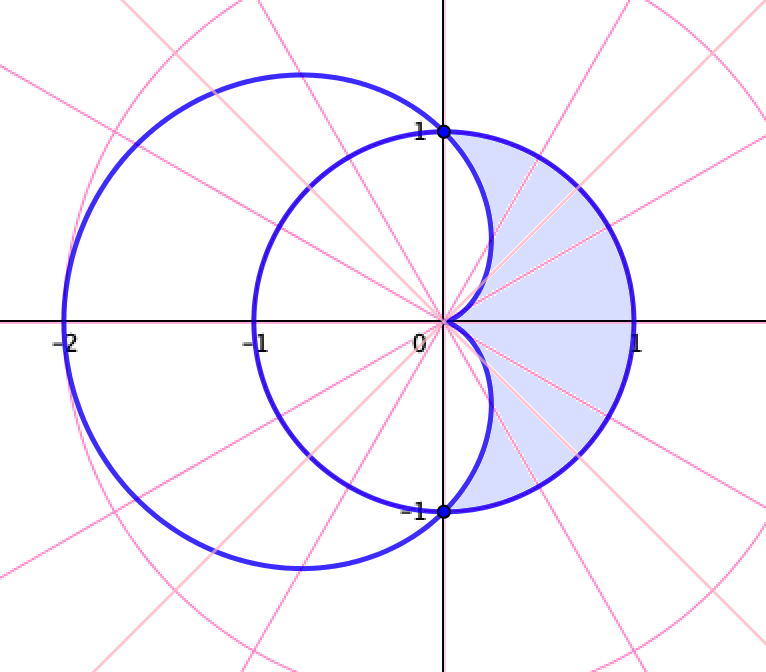
\includegraphics[width=.25\textwidth]{img-polares/polares33.png}
\end{figure}	
\end{multicols}

$A=\displaystyle \int_{-\pi/2}^{\pi/2} \dfrac 1 2 \, \left( 1-(1-\cos \theta)^2 \right) \, \dd \theta =  \int_{-\pi/2}^{\pi/2} (2\cos \theta - \cos^2 \theta)\, \dd \theta =  \int_{-\pi/2}^{\pi/2} \left( 2\cos \theta - \dfrac 1 2 +\dfrac 1 2 \cos 2\theta \right) \, \dd \theta = \left[ 2\sin \theta - \dfrac \theta 2 -\dfrac{\sin 2\theta}2 \right]_{-\pi/2}^{\pi/2}=2-\dfrac \pi 4 \ \ \mathrm{u}^2$


\begin{flushright}\textcolor{teal}{\rule{250pt}{0.2pt}}	\end{flushright} \vspace{5mm}

\vspace{5mm}

\large{\textbf{Longitud de una arco de curva}}\normalsize{:}

\vspace{5mm}

En paramétricas, $\ L=\displaystyle \int_{\theta_1}^{\theta_2} \sqrt{ \left( \dv{x}{\theta} \right)^2 +    \left( \dv{y}{\theta} \right)^2  } \ \dd \theta \ $,  parametrizando,

$r=f(\theta) \to \begin{cases} 
 \ x=r\cos \theta = f(\theta)\cos \theta & \to \displaystyle \dv{x}{\theta}= f'(\theta)\cos \theta - f(\theta)\sin \theta	 \\ \\ 
 \ y=r\sin \theta = f(\theta)\sin \theta & \to \displaystyle \dv{y}{\theta}= f'(\theta)\sin \theta + f(\theta)\cos \theta
 \end{cases}$
 
 $\begin{cases}
\ \displaystyle \left( \dv{x}{\theta} \right)^2 =f'(\theta)^2 \cos^2 \theta +  f(\theta)^2 \sin^2 \theta - 2 f'(\theta) f(\theta) \sin(\theta) \cos\theta \\ \ \displaystyle \left( \dv{y}{\theta} \right)^2 =f'(\theta)^2 \sin^2 \theta +  f(\theta)^2 \cos^2 \theta - 2 f'(\theta) f(\theta) \sin(\theta) \cos\theta
\end{cases}$

Sumando: $\qquad f'^2(\theta)+f^2(\theta)\ = \ f'^2(\theta) + r^2 \ = \ \displaystyle \left( \dv{r}{\theta} \right)^2+r^2$

$$ \boxed{ \ \subrayado{ \ 
L\ = \ \displaystyle \int_{\theta_1}^{\theta_2}{ \sqrt{r^2\, +\, \left( \dv{r}{\theta} \right)^2}\, \dd \theta }
\ } \ }$$




\vspace{5mm}
	
\begin{miejercicio} 
	

Calcula la longitud de la cardioide $r=1-\cos \theta $

 \rule{300pt}{0.2pt}

$\theta \in [0,2\pi]; \quad \displaystyle \dv{r}{\theta}=\sin \theta;\qquad \displaystyle r^2+\left( \dv{r}{\theta} \right)^2=(1-\cos \theta)^2+(\sin \theta)^2=2-2\cos \theta$

$L=\displaystyle \int_0^{2\pi} \sqrt{2-2\cos \theta} \ \dd \theta
= \int_0^{2\pi} \sqrt{4\sin^2 \dfrac \theta 2}\ \dd \theta = \int_0^{2\pi} 2|\sin \dfrac \theta 2|\ \dd \theta = \int_0^{2\pi} 2\sin \dfrac \theta 2 \ \dd \theta =\eval{-4\cos \dfrac \theta 2}_0^{2\pi} = 8\ \mathrm{u}$

\end{miejercicio}

Nota: \hspace{1cm} Hemos usado que $\quad 1-\cos \alpha=2\sin^2 \dfrac \alpha 2 \ $ y que $\ \sin \dfrac \theta 2 \ge 0\ $ cuando $\ \theta \in [0,2\pi]$.


\vspace{5mm}

\section{Cónicas en polares}

\vspace{-5mm}

\begin{tikzpicture}
	\fill [left color=red!50, right color=teal!50] (0,0) rectangle (3.5,.1);
	\fill [left color=teal!50, right color=blue!50] (3.5,0) rectangle (7.5,.1);
	\end{tikzpicture}
\vspace{0.5cm}


%\vspace{5mm}

\normalsize{Las} trayectorias de los cuerpos sometidos a la acción de un campo gravitatorio son elipses, parábolas e hipérbolas que, en coordenadas polares, se pueden expresar por medio de una sola ecuación polar relativamente sencilla.

\vspace{5mm}

En coordenadas rectangulares:
\vspace{-3mm}
\begin{cuadro-naranja}
\tiny{$\qquad \blacksquare \quad $}\normalsize{\emph{Excentricidad}} de la elipse: $\quad \dfrac {x^2}{a^2}+\dfrac{y^2}{b^2}=1 \ , \ \ (a>b):\qquad \boldsymbol{ e=\dfrac c a = \dfrac{\sqrt{a^2-b^2}}{a} }$

\tiny{$\qquad \blacksquare \quad $}\normalsize{\emph{Excentricidad}} de la hipérbola: $\quad \dfrac {x^2}{a^2}-\dfrac{y^2}{b^2}=1 \ : \qquad \boldsymbol{ e=\dfrac c a = \dfrac{\sqrt{a^2+b^2}}{a} }$

\tiny{$\qquad \blacksquare \quad $}\normalsize{\emph{Excentricidad}} de la parábola: $ \quad \boldsymbol{ e=1 }$	
\end{cuadro-naranja}

\textcolor{gris}{Nota: \hspace{1cm} $c=\sqrt{a^2-b^2} \ $ en la elipse, pero $c=\sqrt{a^2+b^2} \ $ en la hipérbola.}

\vspace{5mm}

Una parábola $ \ (y^2=\pm 4cx \ \ \vee \ \ x^2=\pm 4cy ) \ $ tiene un foco $\ F(\pm c, 0 ) \ \ \vee \ \ F(0,\pm c) \  $ y una directriz $ \ ( D:\ y=\mp c \ \ \vee \ \ x=\mp c )\ $.
Una elipse tiene \textbf{dos} focos $\ ( F_1(c,0) \ \ \wedge \ \ F_2(-c,0) \ $ y \textbf{dos} directrices $\ (D_i:\ y=\pm a/e) $

En la parábola se cumple que $\ \boldsymbol {\overline{PF}=1\cdot \overline{PD} } \ $ (\textsf{ecuación foco-directriz}) y se puede demostrar que el la elipse se cumplen las relaciones $ \ \begin{cases} \ \overline{PF_1}=e\cdot \overline{PD_1} \\ \ \overline{PF_2}=e\cdot \overline{PD_2} \end{cases}\, , \ $ donde $e$ es la \emph{excentricidad} de la elipse. Lo mismo ocurre con la hipérbola.

La excentricidad se define como la razón entre distancia entre los focos y la distancia entre los vértices: $\ \boldsymbol e=\dfrac{2c}{2a}= \boldsymbol{ \dfrac c a}$. En la elipse $c<a \ \to \ e<1$, en la hipérbola $c>a \ \to \ e>1$ y para la parábola $c=a \ \to \ e=1$.

La ecuación foco-directriz, $\ \boldsymbol {\overline{PF}=e\cdot \overline{PD}} \, \ $ unifica las tres cónicas (parábola, elipse e hipérbola). 

\begin{cuadro-naranja}
$$\subrayado{ \boldsymbol{
\boxed{ \  \overline{PF} \ = \ e \cdot \ \overline{PD} } \ } \qquad \Rightarrow \quad \begin{cases}
 \ e< 1 \ &\to \ \text{ elipse} \\ 	
  \ e= 1 \ &\to \ \text{ parábola} \\ 
   \ e> 1 \ &\to \ \text{ hipérbola} 
 \end{cases} }$$
 
 \textsf{Podemos definir una \emph{cónica} como el lugar geométrico de los puntos $P$ del plano cuyo cociente de distancias a un punto fijo llamado foco $F$ y a una recta fija llamada directriz $D$ es una cantidad constante llamada excentricidad $e$.}
\vspace{2mm}
\end{cuadro-naranja}
 
 Si $\ e \longrightarrow 1^- \ \rightarrow $ elipse más oblonga; si $\ e\longrightarrow +\infty \ \rightarrow $ hipérbola se convierte en dos rectas paralelas.
 La ecuación foco-directriz se escribe de distinto modo en coordenadas rectangulares según el valor de $e$ pero se escribe como una única ecuación en coordenadas polares.

\begin{figure}[H]
	\centering
	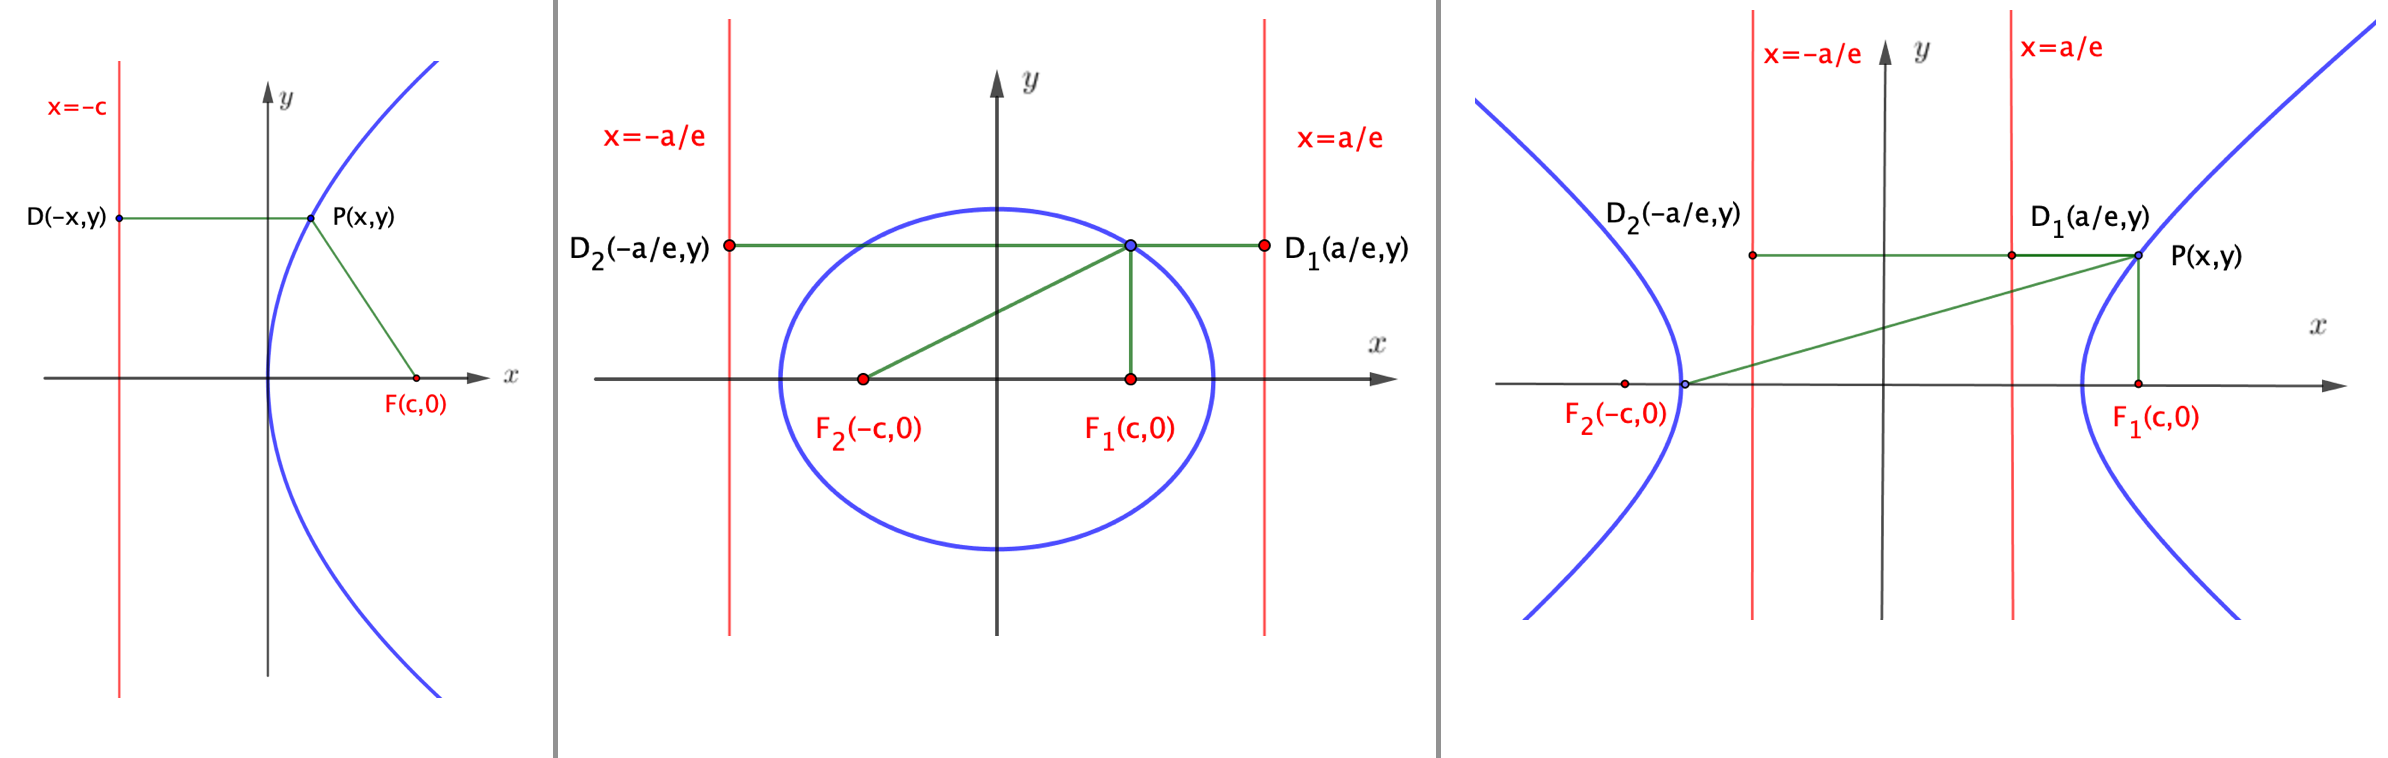
\includegraphics[width=.95\textwidth]{img-polares/polares34.png}
\end{figure}

%\vspace{5mm}
\textbf{\large{Ecuaciones polares de las cónicas}}\normalsize{.}
\vspace{5mm}

\begin{multicols}{2}

De la figura,

ecuación foco-directriz, $\ \overline{PF}=e\cdot \overline{PD} \, : \ $ 

$r=e\, [\, d-r\, \cos(\theta-\theta_0) \, ]$

$r+e\, r\, \cos(\theta-\theta_0)=e\, d$

$\boldsymbol{ \ \subrayado { \ 
r\ = \ \dfrac{e\, d}{1\, +\, e\, \cos (\theta-\theta_0)}
\ } \ }$

\begin{figure}[H]
	\centering
	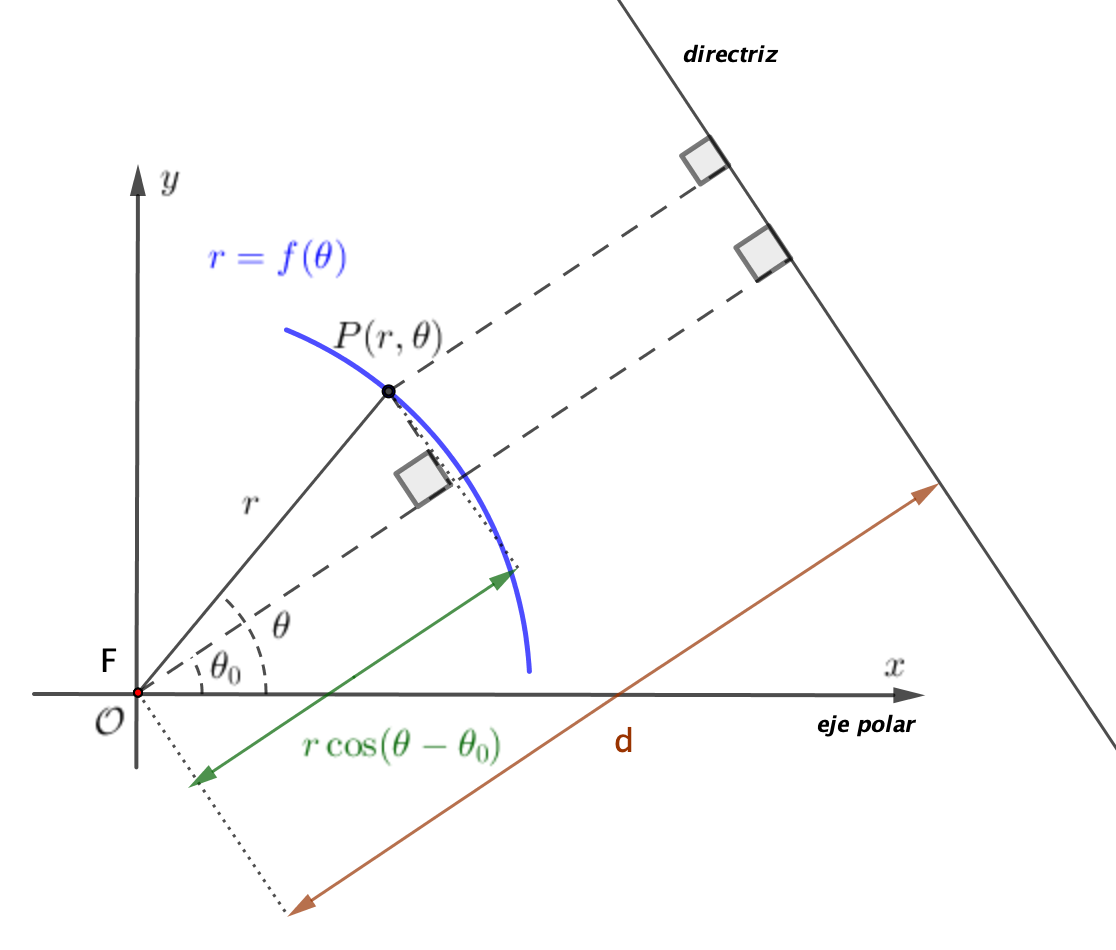
\includegraphics[width=.5\textwidth]{img-polares/polares44.png}
\end{figure}
\end{multicols}

\vspace{-10mm}
\underline{Observaciones}:

\tiny{$ \blacksquare \quad $}\normalsize{$\theta_0=0 \ \to \ r=\dfrac{ed}{1+e\cos \theta}$}
$\qquad \qquad \ \ \ $ \tiny{$ \blacksquare \quad $}\normalsize{$\theta_0=\pi \ \to \ r=\dfrac{ed}{1-e\cos \theta}$}

\tiny{$ \blacksquare \quad $}\normalsize{$\theta_0=\pi/2 \ \to \ r=\dfrac{ed}{1+e\sin \theta}$}
$\qquad \qquad$ \tiny{$ \blacksquare \quad $}\normalsize{$\theta_0=3\pi/2 \ \to \ r=\dfrac{ed}{1-e\sin \theta}$}

\begin{miejercicio}

Graficar $\  r=\dfrac{6}{1+\cos \theta}$ 

 \rule{300pt}{0.2pt}

\begin{multicols}{2}
Por inspección de la ecuación, 

\textcolor{gris}{$\ \qquad \qquad (r=\dfrac{ed}{1+\cos \theta} \ $) },

concluimos que $\ e=1\ $ (coeficiente del coseno), por lo que $\ d=3 \ $. Se trata de una parábola, con el polo en el origen y directriz de ecuación cartesiana $\ x=6 \ $. La parábola va hacia la izquierda.
\begin{figure}[H]
	\centering
	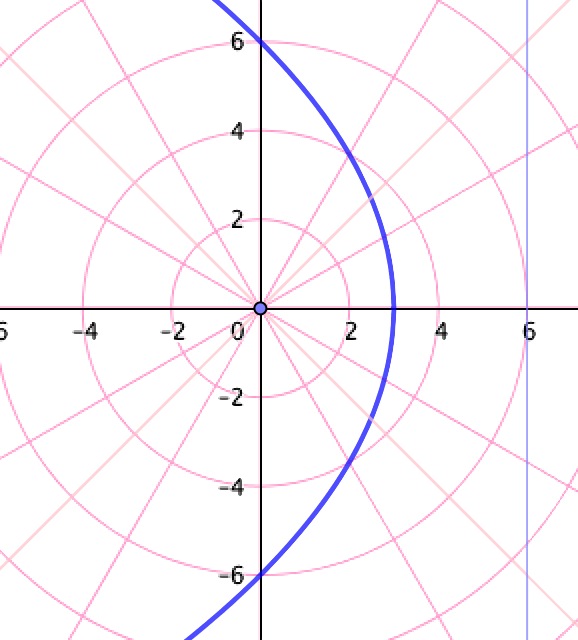
\includegraphics[width=.25\textwidth]{img-polares/polares45.png}
\end{figure}
\vspace{2mm}
\end{multicols}

\end{miejercicio}


\begin{miejercicio} 
	
Graficar $\  r=\dfrac{6}{1-\dfrac 1 2 \sin \theta} $ \textcolor{gris}{$\quad = \ \dfrac{12}{2-\sin \theta}$} 

\rule{300pt}{0.2pt}

\begin{multicols}{2}
Por inspección de la ecuación, 

\textcolor{gris}{$\ \qquad \qquad (r=\dfrac{ed}{1+\cos \theta} \ $) },

concluimos que $\ e=1/2<1\ $ (coeficiente del coseno), por lo que $\ d=12 \ $. Se trata de una elipse, con el polo en el origen y el otro en el eje y ($\pi/2$).
\begin{figure}[H]
	\centering
	\includegraphics[width=.25\textwidth]{img-polares/polares46.png}
\end{figure}
\vspace{2mm}
\end{multicols}

\end{miejercicio}

\begin{miejercicio} 
	

Graficar $\  r=\dfrac{6}{1-2 \sin \theta} $ 

\rule{300pt}{0.2pt}

\begin{multicols}{2}
Por inspección de la ecuación, 

\textcolor{gris}{$\ \qquad \qquad (r=\dfrac{ed}{1+\cos \theta} \ $) },

concluimos que $\ e=2>1\ $ (coeficiente del coseno), por lo que $\ d=3 \ $. Se trata de una hipérbola, con el polo en el origen y el otro en el eje y$^-$ ($3\pi/2$).
\begin{figure}[H]
	\centering
	\includegraphics[width=.25\textwidth]{img-polares/polares47.png}
\end{figure}
\vspace{2mm}
\end{multicols}

\end{miejercicio}	







\begin{comment}

%%%%%%%%%%%%%%%%%%%%%%%%%%%%%%%%%%%. SECCIONES
\chapter{texto}

\begin{tikzpicture}
	\fill [left color=red!50, right color=teal!50] (0,0) rectangle (6.5,.2);
	\fill [left color=teal!50, right color=blue!50] (6.5,0) rectangle (11.5,.2);
	\end{tikzpicture}

\vspace{1cm}
\section{texto}

\begin{tikzpicture}
	\fill [left color=red!50, right color=teal!50] (0,0) rectangle (3.5,.1);
	\fill [left color=teal!50, right color=blue!50] (3.5,0) rectangle (7.5,.1);
	\end{tikzpicture}
\vspace{0.5cm}

\subsection{texto}

\begin{tikzpicture}
	\fill [left color=red!50, right color=teal!50] (0,0) rectangle (3.5,.01);
	\fill [left color=teal!50, right color=blue!50] (3.5,0) rectangle (7.5,.01);
	\end{tikzpicture}
\vspace{0.5cm}


%%%%%%%%%%%%%%%%%%%%%%%%%%%%%%%%%%%. \begin{ ------>. 
detsacado;  cuadro-naranja;  cuadro-gris;  miejercicio (solución extensa);  mipropuesto (solución corta y fuera del cuadro)

%%%%%%%%%%%%%%%%%%%%%%%%%%%%%%%%%%%. CURIOSIDAD
\vspace{1cm}
\color{ForestGreen!80}
\rule{250pt}{0.2pt}
Texto
\vspace{-8mm}
\begin{flushright}
\rule{250pt}{0.2pt}		
\end{flushright}	
\color{black}
\end{comment}





